\documentclass[11pt]{article}

    \usepackage[breakable]{tcolorbox}
    \usepackage{parskip} % Stop auto-indenting (to mimic markdown behaviour)
    
    \usepackage{iftex}
    \ifPDFTeX
    	\usepackage[T1]{fontenc}
    	\usepackage{mathpazo}
    \else
    	\usepackage{fontspec}
    \fi

    % Basic figure setup, for now with no caption control since it's done
    % automatically by Pandoc (which extracts ![](path) syntax from Markdown).
    \usepackage{graphicx}
    % Maintain compatibility with old templates. Remove in nbconvert 6.0
    \let\Oldincludegraphics\includegraphics
    % Ensure that by default, figures have no caption (until we provide a
    % proper Figure object with a Caption API and a way to capture that
    % in the conversion process - todo).
    \usepackage{caption}
    \DeclareCaptionFormat{nocaption}{}
    \captionsetup{format=nocaption,aboveskip=0pt,belowskip=0pt}

    \usepackage{float}
    \floatplacement{figure}{H} % forces figures to be placed at the correct location
    \usepackage{xcolor} % Allow colors to be defined
    \usepackage{enumerate} % Needed for markdown enumerations to work
    \usepackage{geometry} % Used to adjust the document margins
    \usepackage{amsmath} % Equations
    \usepackage{amssymb} % Equations
    \usepackage{textcomp} % defines textquotesingle
    % Hack from http://tex.stackexchange.com/a/47451/13684:
    \AtBeginDocument{%
        \def\PYZsq{\textquotesingle}% Upright quotes in Pygmentized code
    }
    \usepackage{upquote} % Upright quotes for verbatim code
    \usepackage{eurosym} % defines \euro
    \usepackage[mathletters]{ucs} % Extended unicode (utf-8) support
    \usepackage{fancyvrb} % verbatim replacement that allows latex
    \usepackage{grffile} % extends the file name processing of package graphics 
                         % to support a larger range
    \makeatletter % fix for old versions of grffile with XeLaTeX
    \@ifpackagelater{grffile}{2019/11/01}
    {
      % Do nothing on new versions
    }
    {
      \def\Gread@@xetex#1{%
        \IfFileExists{"\Gin@base".bb}%
        {\Gread@eps{\Gin@base.bb}}%
        {\Gread@@xetex@aux#1}%
      }
    }
    \makeatother
    \usepackage[Export]{adjustbox} % Used to constrain images to a maximum size
    \adjustboxset{max size={0.9\linewidth}{0.9\paperheight}}

    % The hyperref package gives us a pdf with properly built
    % internal navigation ('pdf bookmarks' for the table of contents,
    % internal cross-reference links, web links for URLs, etc.)
    \usepackage{hyperref}
    % The default LaTeX title has an obnoxious amount of whitespace. By default,
    % titling removes some of it. It also provides customization options.
    \usepackage{titling}
    \usepackage{longtable} % longtable support required by pandoc >1.10
    \usepackage{booktabs}  % table support for pandoc > 1.12.2
    \usepackage[inline]{enumitem} % IRkernel/repr support (it uses the enumerate* environment)
    \usepackage[normalem]{ulem} % ulem is needed to support strikethroughs (\sout)
                                % normalem makes italics be italics, not underlines
    \usepackage{mathrsfs}
    

    
    % Colors for the hyperref package
    \definecolor{urlcolor}{rgb}{0,.145,.698}
    \definecolor{linkcolor}{rgb}{.71,0.21,0.01}
    \definecolor{citecolor}{rgb}{.12,.54,.11}

    % ANSI colors
    \definecolor{ansi-black}{HTML}{3E424D}
    \definecolor{ansi-black-intense}{HTML}{282C36}
    \definecolor{ansi-red}{HTML}{E75C58}
    \definecolor{ansi-red-intense}{HTML}{B22B31}
    \definecolor{ansi-green}{HTML}{00A250}
    \definecolor{ansi-green-intense}{HTML}{007427}
    \definecolor{ansi-yellow}{HTML}{DDB62B}
    \definecolor{ansi-yellow-intense}{HTML}{B27D12}
    \definecolor{ansi-blue}{HTML}{208FFB}
    \definecolor{ansi-blue-intense}{HTML}{0065CA}
    \definecolor{ansi-magenta}{HTML}{D160C4}
    \definecolor{ansi-magenta-intense}{HTML}{A03196}
    \definecolor{ansi-cyan}{HTML}{60C6C8}
    \definecolor{ansi-cyan-intense}{HTML}{258F8F}
    \definecolor{ansi-white}{HTML}{C5C1B4}
    \definecolor{ansi-white-intense}{HTML}{A1A6B2}
    \definecolor{ansi-default-inverse-fg}{HTML}{FFFFFF}
    \definecolor{ansi-default-inverse-bg}{HTML}{000000}

    % common color for the border for error outputs.
    \definecolor{outerrorbackground}{HTML}{FFDFDF}

    % commands and environments needed by pandoc snippets
    % extracted from the output of `pandoc -s`
    \providecommand{\tightlist}{%
      \setlength{\itemsep}{0pt}\setlength{\parskip}{0pt}}
    \DefineVerbatimEnvironment{Highlighting}{Verbatim}{commandchars=\\\{\}}
    % Add ',fontsize=\small' for more characters per line
    \newenvironment{Shaded}{}{}
    \newcommand{\KeywordTok}[1]{\textcolor[rgb]{0.00,0.44,0.13}{\textbf{{#1}}}}
    \newcommand{\DataTypeTok}[1]{\textcolor[rgb]{0.56,0.13,0.00}{{#1}}}
    \newcommand{\DecValTok}[1]{\textcolor[rgb]{0.25,0.63,0.44}{{#1}}}
    \newcommand{\BaseNTok}[1]{\textcolor[rgb]{0.25,0.63,0.44}{{#1}}}
    \newcommand{\FloatTok}[1]{\textcolor[rgb]{0.25,0.63,0.44}{{#1}}}
    \newcommand{\CharTok}[1]{\textcolor[rgb]{0.25,0.44,0.63}{{#1}}}
    \newcommand{\StringTok}[1]{\textcolor[rgb]{0.25,0.44,0.63}{{#1}}}
    \newcommand{\CommentTok}[1]{\textcolor[rgb]{0.38,0.63,0.69}{\textit{{#1}}}}
    \newcommand{\OtherTok}[1]{\textcolor[rgb]{0.00,0.44,0.13}{{#1}}}
    \newcommand{\AlertTok}[1]{\textcolor[rgb]{1.00,0.00,0.00}{\textbf{{#1}}}}
    \newcommand{\FunctionTok}[1]{\textcolor[rgb]{0.02,0.16,0.49}{{#1}}}
    \newcommand{\RegionMarkerTok}[1]{{#1}}
    \newcommand{\ErrorTok}[1]{\textcolor[rgb]{1.00,0.00,0.00}{\textbf{{#1}}}}
    \newcommand{\NormalTok}[1]{{#1}}
    
    % Additional commands for more recent versions of Pandoc
    \newcommand{\ConstantTok}[1]{\textcolor[rgb]{0.53,0.00,0.00}{{#1}}}
    \newcommand{\SpecialCharTok}[1]{\textcolor[rgb]{0.25,0.44,0.63}{{#1}}}
    \newcommand{\VerbatimStringTok}[1]{\textcolor[rgb]{0.25,0.44,0.63}{{#1}}}
    \newcommand{\SpecialStringTok}[1]{\textcolor[rgb]{0.73,0.40,0.53}{{#1}}}
    \newcommand{\ImportTok}[1]{{#1}}
    \newcommand{\DocumentationTok}[1]{\textcolor[rgb]{0.73,0.13,0.13}{\textit{{#1}}}}
    \newcommand{\AnnotationTok}[1]{\textcolor[rgb]{0.38,0.63,0.69}{\textbf{\textit{{#1}}}}}
    \newcommand{\CommentVarTok}[1]{\textcolor[rgb]{0.38,0.63,0.69}{\textbf{\textit{{#1}}}}}
    \newcommand{\VariableTok}[1]{\textcolor[rgb]{0.10,0.09,0.49}{{#1}}}
    \newcommand{\ControlFlowTok}[1]{\textcolor[rgb]{0.00,0.44,0.13}{\textbf{{#1}}}}
    \newcommand{\OperatorTok}[1]{\textcolor[rgb]{0.40,0.40,0.40}{{#1}}}
    \newcommand{\BuiltInTok}[1]{{#1}}
    \newcommand{\ExtensionTok}[1]{{#1}}
    \newcommand{\PreprocessorTok}[1]{\textcolor[rgb]{0.74,0.48,0.00}{{#1}}}
    \newcommand{\AttributeTok}[1]{\textcolor[rgb]{0.49,0.56,0.16}{{#1}}}
    \newcommand{\InformationTok}[1]{\textcolor[rgb]{0.38,0.63,0.69}{\textbf{\textit{{#1}}}}}
    \newcommand{\WarningTok}[1]{\textcolor[rgb]{0.38,0.63,0.69}{\textbf{\textit{{#1}}}}}
    
    
    % Define a nice break command that doesn't care if a line doesn't already
    % exist.
    \def\br{\hspace*{\fill} \\* }
    % Math Jax compatibility definitions
    \def\gt{>}
    \def\lt{<}
    \let\Oldtex\TeX
    \let\Oldlatex\LaTeX
    \renewcommand{\TeX}{\textrm{\Oldtex}}
    \renewcommand{\LaTeX}{\textrm{\Oldlatex}}
    % Document parameters
    % Document title
    \title{pdf\_submission\_template}
    
    
    
    
    
% Pygments definitions
\makeatletter
\def\PY@reset{\let\PY@it=\relax \let\PY@bf=\relax%
    \let\PY@ul=\relax \let\PY@tc=\relax%
    \let\PY@bc=\relax \let\PY@ff=\relax}
\def\PY@tok#1{\csname PY@tok@#1\endcsname}
\def\PY@toks#1+{\ifx\relax#1\empty\else%
    \PY@tok{#1}\expandafter\PY@toks\fi}
\def\PY@do#1{\PY@bc{\PY@tc{\PY@ul{%
    \PY@it{\PY@bf{\PY@ff{#1}}}}}}}
\def\PY#1#2{\PY@reset\PY@toks#1+\relax+\PY@do{#2}}

\@namedef{PY@tok@w}{\def\PY@tc##1{\textcolor[rgb]{0.73,0.73,0.73}{##1}}}
\@namedef{PY@tok@c}{\let\PY@it=\textit\def\PY@tc##1{\textcolor[rgb]{0.25,0.50,0.50}{##1}}}
\@namedef{PY@tok@cp}{\def\PY@tc##1{\textcolor[rgb]{0.74,0.48,0.00}{##1}}}
\@namedef{PY@tok@k}{\let\PY@bf=\textbf\def\PY@tc##1{\textcolor[rgb]{0.00,0.50,0.00}{##1}}}
\@namedef{PY@tok@kp}{\def\PY@tc##1{\textcolor[rgb]{0.00,0.50,0.00}{##1}}}
\@namedef{PY@tok@kt}{\def\PY@tc##1{\textcolor[rgb]{0.69,0.00,0.25}{##1}}}
\@namedef{PY@tok@o}{\def\PY@tc##1{\textcolor[rgb]{0.40,0.40,0.40}{##1}}}
\@namedef{PY@tok@ow}{\let\PY@bf=\textbf\def\PY@tc##1{\textcolor[rgb]{0.67,0.13,1.00}{##1}}}
\@namedef{PY@tok@nb}{\def\PY@tc##1{\textcolor[rgb]{0.00,0.50,0.00}{##1}}}
\@namedef{PY@tok@nf}{\def\PY@tc##1{\textcolor[rgb]{0.00,0.00,1.00}{##1}}}
\@namedef{PY@tok@nc}{\let\PY@bf=\textbf\def\PY@tc##1{\textcolor[rgb]{0.00,0.00,1.00}{##1}}}
\@namedef{PY@tok@nn}{\let\PY@bf=\textbf\def\PY@tc##1{\textcolor[rgb]{0.00,0.00,1.00}{##1}}}
\@namedef{PY@tok@ne}{\let\PY@bf=\textbf\def\PY@tc##1{\textcolor[rgb]{0.82,0.25,0.23}{##1}}}
\@namedef{PY@tok@nv}{\def\PY@tc##1{\textcolor[rgb]{0.10,0.09,0.49}{##1}}}
\@namedef{PY@tok@no}{\def\PY@tc##1{\textcolor[rgb]{0.53,0.00,0.00}{##1}}}
\@namedef{PY@tok@nl}{\def\PY@tc##1{\textcolor[rgb]{0.63,0.63,0.00}{##1}}}
\@namedef{PY@tok@ni}{\let\PY@bf=\textbf\def\PY@tc##1{\textcolor[rgb]{0.60,0.60,0.60}{##1}}}
\@namedef{PY@tok@na}{\def\PY@tc##1{\textcolor[rgb]{0.49,0.56,0.16}{##1}}}
\@namedef{PY@tok@nt}{\let\PY@bf=\textbf\def\PY@tc##1{\textcolor[rgb]{0.00,0.50,0.00}{##1}}}
\@namedef{PY@tok@nd}{\def\PY@tc##1{\textcolor[rgb]{0.67,0.13,1.00}{##1}}}
\@namedef{PY@tok@s}{\def\PY@tc##1{\textcolor[rgb]{0.73,0.13,0.13}{##1}}}
\@namedef{PY@tok@sd}{\let\PY@it=\textit\def\PY@tc##1{\textcolor[rgb]{0.73,0.13,0.13}{##1}}}
\@namedef{PY@tok@si}{\let\PY@bf=\textbf\def\PY@tc##1{\textcolor[rgb]{0.73,0.40,0.53}{##1}}}
\@namedef{PY@tok@se}{\let\PY@bf=\textbf\def\PY@tc##1{\textcolor[rgb]{0.73,0.40,0.13}{##1}}}
\@namedef{PY@tok@sr}{\def\PY@tc##1{\textcolor[rgb]{0.73,0.40,0.53}{##1}}}
\@namedef{PY@tok@ss}{\def\PY@tc##1{\textcolor[rgb]{0.10,0.09,0.49}{##1}}}
\@namedef{PY@tok@sx}{\def\PY@tc##1{\textcolor[rgb]{0.00,0.50,0.00}{##1}}}
\@namedef{PY@tok@m}{\def\PY@tc##1{\textcolor[rgb]{0.40,0.40,0.40}{##1}}}
\@namedef{PY@tok@gh}{\let\PY@bf=\textbf\def\PY@tc##1{\textcolor[rgb]{0.00,0.00,0.50}{##1}}}
\@namedef{PY@tok@gu}{\let\PY@bf=\textbf\def\PY@tc##1{\textcolor[rgb]{0.50,0.00,0.50}{##1}}}
\@namedef{PY@tok@gd}{\def\PY@tc##1{\textcolor[rgb]{0.63,0.00,0.00}{##1}}}
\@namedef{PY@tok@gi}{\def\PY@tc##1{\textcolor[rgb]{0.00,0.63,0.00}{##1}}}
\@namedef{PY@tok@gr}{\def\PY@tc##1{\textcolor[rgb]{1.00,0.00,0.00}{##1}}}
\@namedef{PY@tok@ge}{\let\PY@it=\textit}
\@namedef{PY@tok@gs}{\let\PY@bf=\textbf}
\@namedef{PY@tok@gp}{\let\PY@bf=\textbf\def\PY@tc##1{\textcolor[rgb]{0.00,0.00,0.50}{##1}}}
\@namedef{PY@tok@go}{\def\PY@tc##1{\textcolor[rgb]{0.53,0.53,0.53}{##1}}}
\@namedef{PY@tok@gt}{\def\PY@tc##1{\textcolor[rgb]{0.00,0.27,0.87}{##1}}}
\@namedef{PY@tok@err}{\def\PY@bc##1{{\setlength{\fboxsep}{\string -\fboxrule}\fcolorbox[rgb]{1.00,0.00,0.00}{1,1,1}{\strut ##1}}}}
\@namedef{PY@tok@kc}{\let\PY@bf=\textbf\def\PY@tc##1{\textcolor[rgb]{0.00,0.50,0.00}{##1}}}
\@namedef{PY@tok@kd}{\let\PY@bf=\textbf\def\PY@tc##1{\textcolor[rgb]{0.00,0.50,0.00}{##1}}}
\@namedef{PY@tok@kn}{\let\PY@bf=\textbf\def\PY@tc##1{\textcolor[rgb]{0.00,0.50,0.00}{##1}}}
\@namedef{PY@tok@kr}{\let\PY@bf=\textbf\def\PY@tc##1{\textcolor[rgb]{0.00,0.50,0.00}{##1}}}
\@namedef{PY@tok@bp}{\def\PY@tc##1{\textcolor[rgb]{0.00,0.50,0.00}{##1}}}
\@namedef{PY@tok@fm}{\def\PY@tc##1{\textcolor[rgb]{0.00,0.00,1.00}{##1}}}
\@namedef{PY@tok@vc}{\def\PY@tc##1{\textcolor[rgb]{0.10,0.09,0.49}{##1}}}
\@namedef{PY@tok@vg}{\def\PY@tc##1{\textcolor[rgb]{0.10,0.09,0.49}{##1}}}
\@namedef{PY@tok@vi}{\def\PY@tc##1{\textcolor[rgb]{0.10,0.09,0.49}{##1}}}
\@namedef{PY@tok@vm}{\def\PY@tc##1{\textcolor[rgb]{0.10,0.09,0.49}{##1}}}
\@namedef{PY@tok@sa}{\def\PY@tc##1{\textcolor[rgb]{0.73,0.13,0.13}{##1}}}
\@namedef{PY@tok@sb}{\def\PY@tc##1{\textcolor[rgb]{0.73,0.13,0.13}{##1}}}
\@namedef{PY@tok@sc}{\def\PY@tc##1{\textcolor[rgb]{0.73,0.13,0.13}{##1}}}
\@namedef{PY@tok@dl}{\def\PY@tc##1{\textcolor[rgb]{0.73,0.13,0.13}{##1}}}
\@namedef{PY@tok@s2}{\def\PY@tc##1{\textcolor[rgb]{0.73,0.13,0.13}{##1}}}
\@namedef{PY@tok@sh}{\def\PY@tc##1{\textcolor[rgb]{0.73,0.13,0.13}{##1}}}
\@namedef{PY@tok@s1}{\def\PY@tc##1{\textcolor[rgb]{0.73,0.13,0.13}{##1}}}
\@namedef{PY@tok@mb}{\def\PY@tc##1{\textcolor[rgb]{0.40,0.40,0.40}{##1}}}
\@namedef{PY@tok@mf}{\def\PY@tc##1{\textcolor[rgb]{0.40,0.40,0.40}{##1}}}
\@namedef{PY@tok@mh}{\def\PY@tc##1{\textcolor[rgb]{0.40,0.40,0.40}{##1}}}
\@namedef{PY@tok@mi}{\def\PY@tc##1{\textcolor[rgb]{0.40,0.40,0.40}{##1}}}
\@namedef{PY@tok@il}{\def\PY@tc##1{\textcolor[rgb]{0.40,0.40,0.40}{##1}}}
\@namedef{PY@tok@mo}{\def\PY@tc##1{\textcolor[rgb]{0.40,0.40,0.40}{##1}}}
\@namedef{PY@tok@ch}{\let\PY@it=\textit\def\PY@tc##1{\textcolor[rgb]{0.25,0.50,0.50}{##1}}}
\@namedef{PY@tok@cm}{\let\PY@it=\textit\def\PY@tc##1{\textcolor[rgb]{0.25,0.50,0.50}{##1}}}
\@namedef{PY@tok@cpf}{\let\PY@it=\textit\def\PY@tc##1{\textcolor[rgb]{0.25,0.50,0.50}{##1}}}
\@namedef{PY@tok@c1}{\let\PY@it=\textit\def\PY@tc##1{\textcolor[rgb]{0.25,0.50,0.50}{##1}}}
\@namedef{PY@tok@cs}{\let\PY@it=\textit\def\PY@tc##1{\textcolor[rgb]{0.25,0.50,0.50}{##1}}}

\def\PYZbs{\char`\\}
\def\PYZus{\char`\_}
\def\PYZob{\char`\{}
\def\PYZcb{\char`\}}
\def\PYZca{\char`\^}
\def\PYZam{\char`\&}
\def\PYZlt{\char`\<}
\def\PYZgt{\char`\>}
\def\PYZsh{\char`\#}
\def\PYZpc{\char`\%}
\def\PYZdl{\char`\$}
\def\PYZhy{\char`\-}
\def\PYZsq{\char`\'}
\def\PYZdq{\char`\"}
\def\PYZti{\char`\~}
% for compatibility with earlier versions
\def\PYZat{@}
\def\PYZlb{[}
\def\PYZrb{]}
\makeatother


    % For linebreaks inside Verbatim environment from package fancyvrb. 
    \makeatletter
        \newbox\Wrappedcontinuationbox 
        \newbox\Wrappedvisiblespacebox 
        \newcommand*\Wrappedvisiblespace {\textcolor{red}{\textvisiblespace}} 
        \newcommand*\Wrappedcontinuationsymbol {\textcolor{red}{\llap{\tiny$\m@th\hookrightarrow$}}} 
        \newcommand*\Wrappedcontinuationindent {3ex } 
        \newcommand*\Wrappedafterbreak {\kern\Wrappedcontinuationindent\copy\Wrappedcontinuationbox} 
        % Take advantage of the already applied Pygments mark-up to insert 
        % potential linebreaks for TeX processing. 
        %        {, <, #, %, $, ' and ": go to next line. 
        %        _, }, ^, &, >, - and ~: stay at end of broken line. 
        % Use of \textquotesingle for straight quote. 
        \newcommand*\Wrappedbreaksatspecials {% 
            \def\PYGZus{\discretionary{\char`\_}{\Wrappedafterbreak}{\char`\_}}% 
            \def\PYGZob{\discretionary{}{\Wrappedafterbreak\char`\{}{\char`\{}}% 
            \def\PYGZcb{\discretionary{\char`\}}{\Wrappedafterbreak}{\char`\}}}% 
            \def\PYGZca{\discretionary{\char`\^}{\Wrappedafterbreak}{\char`\^}}% 
            \def\PYGZam{\discretionary{\char`\&}{\Wrappedafterbreak}{\char`\&}}% 
            \def\PYGZlt{\discretionary{}{\Wrappedafterbreak\char`\<}{\char`\<}}% 
            \def\PYGZgt{\discretionary{\char`\>}{\Wrappedafterbreak}{\char`\>}}% 
            \def\PYGZsh{\discretionary{}{\Wrappedafterbreak\char`\#}{\char`\#}}% 
            \def\PYGZpc{\discretionary{}{\Wrappedafterbreak\char`\%}{\char`\%}}% 
            \def\PYGZdl{\discretionary{}{\Wrappedafterbreak\char`\$}{\char`\$}}% 
            \def\PYGZhy{\discretionary{\char`\-}{\Wrappedafterbreak}{\char`\-}}% 
            \def\PYGZsq{\discretionary{}{\Wrappedafterbreak\textquotesingle}{\textquotesingle}}% 
            \def\PYGZdq{\discretionary{}{\Wrappedafterbreak\char`\"}{\char`\"}}% 
            \def\PYGZti{\discretionary{\char`\~}{\Wrappedafterbreak}{\char`\~}}% 
        } 
        % Some characters . , ; ? ! / are not pygmentized. 
        % This macro makes them "active" and they will insert potential linebreaks 
        \newcommand*\Wrappedbreaksatpunct {% 
            \lccode`\~`\.\lowercase{\def~}{\discretionary{\hbox{\char`\.}}{\Wrappedafterbreak}{\hbox{\char`\.}}}% 
            \lccode`\~`\,\lowercase{\def~}{\discretionary{\hbox{\char`\,}}{\Wrappedafterbreak}{\hbox{\char`\,}}}% 
            \lccode`\~`\;\lowercase{\def~}{\discretionary{\hbox{\char`\;}}{\Wrappedafterbreak}{\hbox{\char`\;}}}% 
            \lccode`\~`\:\lowercase{\def~}{\discretionary{\hbox{\char`\:}}{\Wrappedafterbreak}{\hbox{\char`\:}}}% 
            \lccode`\~`\?\lowercase{\def~}{\discretionary{\hbox{\char`\?}}{\Wrappedafterbreak}{\hbox{\char`\?}}}% 
            \lccode`\~`\!\lowercase{\def~}{\discretionary{\hbox{\char`\!}}{\Wrappedafterbreak}{\hbox{\char`\!}}}% 
            \lccode`\~`\/\lowercase{\def~}{\discretionary{\hbox{\char`\/}}{\Wrappedafterbreak}{\hbox{\char`\/}}}% 
            \catcode`\.\active
            \catcode`\,\active 
            \catcode`\;\active
            \catcode`\:\active
            \catcode`\?\active
            \catcode`\!\active
            \catcode`\/\active 
            \lccode`\~`\~ 	
        }
    \makeatother

    \let\OriginalVerbatim=\Verbatim
    \makeatletter
    \renewcommand{\Verbatim}[1][1]{%
        %\parskip\z@skip
        \sbox\Wrappedcontinuationbox {\Wrappedcontinuationsymbol}%
        \sbox\Wrappedvisiblespacebox {\FV@SetupFont\Wrappedvisiblespace}%
        \def\FancyVerbFormatLine ##1{\hsize\linewidth
            \vtop{\raggedright\hyphenpenalty\z@\exhyphenpenalty\z@
                \doublehyphendemerits\z@\finalhyphendemerits\z@
                \strut ##1\strut}%
        }%
        % If the linebreak is at a space, the latter will be displayed as visible
        % space at end of first line, and a continuation symbol starts next line.
        % Stretch/shrink are however usually zero for typewriter font.
        \def\FV@Space {%
            \nobreak\hskip\z@ plus\fontdimen3\font minus\fontdimen4\font
            \discretionary{\copy\Wrappedvisiblespacebox}{\Wrappedafterbreak}
            {\kern\fontdimen2\font}%
        }%
        
        % Allow breaks at special characters using \PYG... macros.
        \Wrappedbreaksatspecials
        % Breaks at punctuation characters . , ; ? ! and / need catcode=\active 	
        \OriginalVerbatim[#1,codes*=\Wrappedbreaksatpunct]%
    }
    \makeatother

    % Exact colors from NB
    \definecolor{incolor}{HTML}{303F9F}
    \definecolor{outcolor}{HTML}{D84315}
    \definecolor{cellborder}{HTML}{CFCFCF}
    \definecolor{cellbackground}{HTML}{F7F7F7}
    
    % prompt
    \makeatletter
    \newcommand{\boxspacing}{\kern\kvtcb@left@rule\kern\kvtcb@boxsep}
    \makeatother
    \newcommand{\prompt}[4]{
        {\ttfamily\llap{{\color{#2}[#3]:\hspace{3pt}#4}}\vspace{-\baselineskip}}
    }
    

    
    % Prevent overflowing lines due to hard-to-break entities
    \sloppy 
    % Setup hyperref package
    \hypersetup{
      breaklinks=true,  % so long urls are correctly broken across lines
      colorlinks=true,
      urlcolor=urlcolor,
      linkcolor=linkcolor,
      citecolor=citecolor,
      }
    % Slightly bigger margins than the latex defaults
    
    \geometry{verbose,tmargin=1in,bmargin=1in,lmargin=1in,rmargin=1in}
    
    

\begin{document}
    
    \maketitle
    
    

    
    \hypertarget{question-1-homography-theory}{%
\subsection{Question 1: Homography
Theory}\label{question-1-homography-theory}}

Suppose we have two cameras \(\mathbf{C}_1\) and \(\mathbf{C}_2\)
looking at a common plane \(\Pi\) in 3D space. Any 3D point
\(\mathbf{P}\) on \(\Pi\) generates a projected 2D point located at
\(\mathbf{p} \equiv (u_1,v_1,1)^T\) on the first camera \(\mathbf{C}_1\)
and \(\mathbf{q} \equiv (u_2,v_2,1)^T\) on the second camera
\(\mathbf{C}_2\). Since \(\mathbf{P}\) is confined to the plane \(\Pi\),
we expect that there is a relationship between \(\mathbf{p}\) and
\(\mathbf{q}\). In particular, there exists a common 3 \(\times\) 3
matrix \(\mathbf{H}\), so that for any \(\mathbf{p}\) and
\(\mathbf{q}\), the following conditions holds: \begin{equation}
\mathbf{p \equiv Hq}
\label{eq:homography}
\end{equation} We call this relationship \textbf{planar homography}.
Recall that both \(\mathbf{p}\) and \(\mathbf{q}\) are in homogeneous
coordinates and the equality \(\equiv\) means \(\mathbf{p}\) is
proportional to \(\mathbf{Hq}\) (recall homogeneous coordinates). It
turns out this relationship is also true for cameras that are related by
pure rotation without the planar constraint.

    \hypertarget{homography-5-points}{%
\subsubsection{1.1 Homography (5 points)}\label{homography-5-points}}

Prove that there exists an \(\mathbf{H}\) that satisfies
\(\mathbf{p \equiv Hq}\) given two \({3 \times 4}\) camera projection
matrices \(\mathbf{M_1}\) and \(\mathbf{M_2}\) corresponding to cameras
\(\mathbf{C_1}\), \(\mathbf{C_2}\) and a plane \(\Pi\). Do not produce
an actual algebraic expression for \(\mathbf{H}\). All we are asking for
is a proof of the existence of \(\mathbf{H}\).

\emph{Note: A degenerate case may happen when the plane \(\Pi\) contains
both cameras' centers, in which case there are infinite choices of
\(\mathbf{H}\) satisfying \(\mathbf{p \equiv Hq}\). You can ignore this
case in your answer.}

    \begin{center}\rule{0.5\linewidth}{0.5pt}\end{center}

Consider the projection of 3D homogeneous point \(\mathbf{P}\) on plane
\(\mathbf{\Pi}\) to the two camera planes as \(\mathbf{p}\) and
\(\mathbf{q}\)

\[\therefore \mathbf{p \equiv M_1P}\]
\[\therefore \mathbf{q \equiv M_2P}\]

From the second equation,

\[\mathbf{P \equiv M_2^{-1}q}\]

Note: \(\mathbf{M_2^{-1}}\) will be of the shape 4x3. Only then can
\(\mathbf{M_2^{-1}M_2 = I}\)

Substituting the value of \(\mathbf{P}\) in first equation

\[\therefore \mathbf{p \equiv M_1M_2^{-1}q}\]

Therefore, it can be seen that there exists a homography
\(\mathbf{H = M_1M_2^{-1}}\) that satisfies \(\mathbf{p \equiv Hq}\)

\begin{center}\rule{0.5\linewidth}{0.5pt}\end{center}

    \hypertarget{homography-under-rotation-5-points}{%
\subsubsection{1.2 Homography under rotation (5
points)}\label{homography-under-rotation-5-points}}

Prove that there exists a homography \(\mathbf{H}\) that satisfies
\(\mathbf{p_1} \equiv \mathbf{Hp_2}\), given two cameras separated by a
pure rotation. That is, for camera 1,
\(\mathbf{p_1} = \mathbf{K_1} \begin{bmatrix} \mathbf{I} & \mathbf{0} \end{bmatrix} \mathbf{P}\)
and for camera 2,
\(\mathbf{p_2} = \mathbf{K_2} \begin{bmatrix}\mathbf{R} & \mathbf{0} \end{bmatrix} \mathbf{P}\).
Note that \(\mathbf{K_1}\) and \(\mathbf{K_2}\) are the \(3 \times 3\)
intrinsic matrices of the two cameras and are different. \(\mathbf{I}\)
is \(3 \times 3\) identity matrix, \(\mathbf{0}\) is a \(3\times1\) zero
vector and \(\mathbf{P}\) is the homogeneous coordinate of a point in 3D
space. \(\mathbf{R}\) is the \(3 \times 3\) rotation matrix of the
camera.

    \begin{center}\rule{0.5\linewidth}{0.5pt}\end{center}

Writing homogeneous coordinate,
\(\mathbf{P} = \begin{bmatrix} \mathbf{X} \\ 1\end{bmatrix}\) where
\(\mathbf{X}\) are the 3D world coordinates.

\[\therefore \mathbf{p_1} \equiv \mathbf{K_1} \begin{bmatrix} \mathbf{I} & \mathbf{0} \end{bmatrix}\begin{bmatrix} \mathbf{X} \\ 1\end{bmatrix} \equiv \mathbf{K_1}\mathbf{X}\]

\[\therefore \mathbf{p_2} \equiv \mathbf{K_2} \begin{bmatrix} \mathbf{R} & \mathbf{0} \end{bmatrix}\begin{bmatrix} \mathbf{X} \\ 1\end{bmatrix} \equiv \mathbf{K_2}\mathbf{R}\mathbf{X}\]

From the second equation,
\[\mathbf{X} \equiv (\mathbf{K_2}\mathbf{R})^{-1}\mathbf{p_2}\]

Substituting this in the first equation,

\[\therefore \mathbf{p_1} \equiv \mathbf{K_1}\mathbf{X} = \mathbf{K_1}(\mathbf{K_2}\mathbf{R})^{-1}\mathbf{p_2}\]
\[\therefore \mathbf{p_1} \equiv \mathbf{K_1}\mathbf{R}^{-1}\mathbf{K_2}^{-1}\mathbf{p_2}\]

where \(\mathbf{K_1}\mathbf{R}^{-1}\mathbf{K_2}^{-1}\) is a 3x3 matrix.

Hence, can be seen that there exists a 3x3 homography
(\(\mathbf{H} = \mathbf{K_1}\mathbf{R}^{-1}\mathbf{K_2}^{-1}\) ) from
\(\mathbf{p_2}\) to \(\mathbf{p_1}\)

\begin{center}\rule{0.5\linewidth}{0.5pt}\end{center}

    \hypertarget{correspondences-10-points}{%
\subsubsection{1.3 Correspondences (10
points)}\label{correspondences-10-points}}

Let \(\mathbf{x_1}\) be a set of points in an image and \(\mathbf{x_2}\)
be the set of corresponding points in an image taken by another camera.
Suppose there exists a homography \(\mathbf{H}\) such that:
\(\mathbf{x^i_1} \equiv \mathbf{Hx^i_2}\quad(i \in \{1\dots N\})\) where
\(\mathbf{x^i_1} = \left[\begin{matrix}x^i_1 & y^i_1 & 1\end{matrix}\right]^T\)
are in homogenous coordinates, \(\mathbf{x_1^i \in \mathbf{x_1}}\) and
\(\mathbf{H}\) is a \(3 \times 3\) matrix. For each point pair, this
relation can be rewritten as \begin{equation*}
\mathbf{A_ih} = 0
\end{equation*} where \(\mathbf{h}\) is a column vector reshaped from
\(\mathbf{H}\), and \(\mathbf{A_i}\) is a matrix with elements derived
from the points \(\mathbf{x^i_1}\) and \(\mathbf{x^i_2}\). This can help
calculate \textbf{H} from the given point correspondences.

\begin{itemize}
\item
  How many degrees of freedom does \(\mathbf{h}\) have? (3 points)
\item
  How many point pairs are required to solve \(\mathbf{h}\)? (2 points)
\item
  Derive \(\mathbf{A_i}\). (5 points)
\end{itemize}

    \begin{center}\rule{0.5\linewidth}{0.5pt}\end{center}

\textbf{h} has 8 degrees of freedom. So, the number of point pairs
required to solve for \textbf{h} is 4.

Given, \(\mathbf{x^i_1} \equiv \mathbf{Hx^i_2}\)

\[ \begin{bmatrix}
x^i_1 \\
y^i_1 \\
1
\end{bmatrix} \equiv \begin{bmatrix}
h11 & h12 & h13 \\
h21 & h22 & h23 \\
h31 & h32 & h33 
\end{bmatrix}\begin{bmatrix}
x^i_2 \\
y^i_2 \\
1
\end{bmatrix}\]

Simplifying RHS

\[ \begin{bmatrix}
h11 & h12 & h13 \\
h21 & h22 & h23 \\
h31 & h32 & h33 
\end{bmatrix}\begin{bmatrix}
x^i_2 \\
y^i_2 \\
1
\end{bmatrix} = \begin{bmatrix}
h11 * x^i_2 + h12 * y^i_2 + h13\\
h21 * x^i_2 + h22 * y^i_2 + h23\\
h31 * x^i_2 + h32 * y^i_2 + h33\\
\end{bmatrix} \]

In order for this to match this to \(\mathbf{x^i_1}\), need to make the
last element 1

\[\begin{bmatrix}
x^i_1 \\
y^i_1 \\
1
\end{bmatrix} = \begin{bmatrix}
\frac{h11 * x^i_2 + h12 * y^i_2 + h13}{h31 * x^i_2 + h32 * y^i_2 + h33}\\
\frac{h21 * x^i_2 + h22 * y^i_2 + h23}{h31 * x^i_2 + h32 * y^i_2 + h33}\\
1\\
\end{bmatrix}\]

\[\therefore x^i_1 = \frac{h11 * x^i_2 + h12 * y^i_2 + h13}{h31 * x^i_2 + h32 * y^i_2 + h33}\]
\[\therefore y^i_1 = \frac{h21 * x^i_2 + h22 * y^i_2 + h23}{h31 * x^i_2 + h32 * y^i_2 + h33}\]

\[\therefore (h31 * x^i_2 + h32 * y^i_2 + h33)x^i_1 = h11 * x^i_2 + h12 * y^i_2 + h13\]
\[\therefore (h31 * x^i_2 + h32 * y^i_2 + h33)y^i_1 = h21 * x^i_2 + h22 * y^i_2 + h23\]

\[\therefore - h11 * x^i_2 - h12 * y^i_2 - h13 + x^i_1x^i_2 * h31 + x^i_1y^i_2 * h32 + x^i_1 * h33 = 0 \]
\[\therefore - h21 * x^i_2 - h22 * y^i_2 - h23 + y^i_1x^i_2 * h31 + y^i_1y^i_2 * h32 + y^i_1 * h33 = 0 \]

Writing this in matrix form,

\[
\begin{bmatrix}
- x^i_2 & - y^i_2 & -1 & 0 & 0 & 0 x^i_1x^i_2 & x^i_1y^i_2 & x^i_1\\
0 & 0 & 0 & - x^i_2 & - y^i_2 & -1 & y^i_1x^i_2 & y^i_1y^i_2 & y^i_1\\
\end{bmatrix}
\begin{bmatrix}
h11\\
h12\\
h13\\
h21\\
h22\\
h23\\
h31\\
h32\\
h33
\end{bmatrix} = \begin{bmatrix}0\\0\end{bmatrix}\]

Hence, the matrix, \[A_i = \begin{bmatrix}
- x^i_2 & - y^i_2 & -1 & 0 & 0 & 0 x^i_1x^i_2 & x^i_1y^i_2 & x^i_1\\
0 & 0 & 0 & - x^i_2 & - y^i_2 & -1 & y^i_1x^i_2 & y^i_1y^i_2 & y^i_1\\
\end{bmatrix}\]

\begin{center}\rule{0.5\linewidth}{0.5pt}\end{center}

    \hypertarget{understanding-homographies-under-rotation-5-points}{%
\subsubsection{1.4 Understanding homographies under rotation (5
points)}\label{understanding-homographies-under-rotation-5-points}}

Suppose that a camera is rotating about its center \(\mathbf{C}\),
keeping the intrinsic parameters \(\mathbf{K}\) constant. Let
\(\mathbf{H}\) be the homography that maps the view from one camera
orientation to the view at a second orientation. Let \(\theta\) be the
angle of rotation between the two. Show that \(\mathbf{H^2}\) is the
homography corresponding to a rotation of 2\(\theta\). Please limit your
answer within a couple of lines. A lengthy proof indicates that you're
doing something too complicated (or wrong).

    \begin{center}\rule{0.5\linewidth}{0.5pt}\end{center}

Considering that the camera's only being rotated around its center,
\(\mathbf{H}\) would be of the form

\[ \mathbf{H} =
\begin{bmatrix}
\cos(\theta) & -\sin(\theta) & 0\\
\sin(\theta) & \cos(\theta) & 0\\
0 & 0 & 1\\
\end{bmatrix} \]

Computing, \(\mathbf{H}^2\)

\[ \mathbf{H}^2 =
\begin{bmatrix}
\cos(\theta) & -\sin(\theta) & 0\\
\sin(\theta) & \cos(\theta) & 0\\
0 & 0 & 1\\
\end{bmatrix}\begin{bmatrix}
\cos(\theta) & -\sin(\theta) & 0\\
\sin(\theta) & \cos(\theta) & 0\\
0 & 0 & 1\\
\end{bmatrix} = \begin{bmatrix}
\cos^2(\theta) - \sin^2(\theta) & -(2\sin(\theta)\cos(\theta)) & 0\\
2\sin(\theta)\cos(\theta)) & \cos^2(\theta) - \sin^2(\theta) & 0\\
0 & 0 & 1\\
\end{bmatrix} = \begin{bmatrix}
\cos(2\theta) & -\sin(2\theta) & 0\\
\sin(2\theta) & \cos(2\theta) & 0\\
0 & 0 & 1\\
\end{bmatrix} \]

Therefore, \(\mathbf{H}^2\) is the homography corresponding to a
rotation of \(2\theta\).

\begin{center}\rule{0.5\linewidth}{0.5pt}\end{center}

    \hypertarget{limitations-of-the-planar-homography-2-points}{%
\subsubsection{1.5 Limitations of the planar homography (2
points)}\label{limitations-of-the-planar-homography-2-points}}

Why is the planar homography not completely sufficient to map any
arbitrary scene image to another viewpoint? State your answer concisely
in one or two sentences.

    \begin{center}\rule{0.5\linewidth}{0.5pt}\end{center}

This expects scene points to lie on a plane which might not always be
possible when there's a significant depth involved. Besides that, a
translation could lead to an occluded viewpoint from which the object of
interest/scene is no longer completely visible.

\begin{center}\rule{0.5\linewidth}{0.5pt}\end{center}

    \hypertarget{behavior-of-lines-under-perspective-projections-3-points}{%
\subsubsection{1.6 Behavior of lines under perspective projections (3
points)}\label{behavior-of-lines-under-perspective-projections-3-points}}

We stated in class that perspective projection preserves lines (a line
in 3D is projected to a line in 2D). Verify algebraically that this is
the case, i.e., verify that the projection \(\mathbf{P}\) in
\(\mathbf{x} = \mathbf{PX}\) preserves lines.

    \begin{center}\rule{0.5\linewidth}{0.5pt}\end{center}

Consider the 3D line to be given by \((x_0, y_0, z_0) + t(a, b, c)\)
where \((a, b, c)\) represent the direction vector, \((x_0, y_0, z_0)\)
represents one point lying on the line and \(t \in \mathbb{R}\) is the
stepping variable that helps satisfy all points lying on this line.

\[\therefore \mathbf{X} = \begin{bmatrix} t*a + x_0 \\t*b + y_0 \\ t*c + z_0 \end{bmatrix}\]

Also, the projection matrix can be broken down into intrinsic and
extrinsic parameter matrices. Assuming that there's no rotation or
translation,

\[\mathbf{x} \equiv 
\alpha \begin{bmatrix} f_x & 0 & o_x \\ 0 & f_y & o_y \\ 0 & 0 & 1\end{bmatrix}
\begin{bmatrix} t*a + x_0 \\t*b + y_0 \\ t*c + z_0 \end{bmatrix}\]

where \(\alpha\) is the scaling factor

\[\mathbf{x} \equiv 
\alpha \begin{bmatrix} f_x * (t*a + x_0) + o_x * (t*c + z_0) \\f_y * (t*b + y_0) + o_y * (t*c + z_0) \\ t*c + z_0 \end{bmatrix}\]

Making these homogeneous

\[\mathbf{x} =
\alpha \begin{bmatrix} \frac{f_x * (t*a + x_0) + o_x * (t*c + z_0)}{t*c + z_0} \\\frac{f_y * (t*b + y_0) + o_y * (t*c + z_0)}{t*c + z_0} \\ 1 \end{bmatrix}\]

\[\therefore x = \alpha * f_x * \frac{t*a + x_0}{t*c + z_0} + \alpha * o_x\]
\[\therefore y = \alpha * f_y * \frac{t*b + y_0}{t*c + z_0} + \alpha * o_y\]

Now, consider 2 3-D points lying on the 3-D line -
\((x_0, y_0, z_0) + t_1(a, b, c)\) and
\((x_0, y_0, z_0) + t_2(a, b, c)\)

The corresponding 2D coordinates would be given by

\[\therefore x_1 = \alpha * f_x * \frac{t_1*a + x_0}{t_1*c + z_0} + \alpha * o_x\]
\[\therefore y_1 = \alpha * f_y * \frac{t_1*b + y_0}{t_1*c + z_0} + \alpha * o_y\]

and

\[\therefore x_2 = \alpha * f_x * \frac{t_2*a + x_0}{t_2*c + z_0} + \alpha * o_x\]
\[\therefore y_2 = \alpha * f_y * \frac{t_2*b + y_0}{t_2*c + z_0} + \alpha * o_y\]

Finding the slope of the line between these 2 points

\[m = \frac{y_2 - y_1}{x_2 - x_1} = \frac{\left[\alpha * f_y * \frac{t_2*b + y_0}{t_2*c + z_0} + \alpha * o_y\right] - \left[\alpha * f_y * \frac{t_1*b + y_0}{t_1*c + z_0} + \alpha * o_y\right]}{\left[\alpha * f_x * \frac{t_2*a + x_0}{t_2*c + z_0} + \alpha * o_x \right]- \left[\alpha * f_x * \frac{t_1*a + x_0}{t_1*c + z_0} + \alpha * o_x\right]} \]

Simplifying,

\[m = \frac{\left[f_y * (t_2*b + y_0)(t_1*c + z_0)\right] - \left[f_y * (t_1*b + y_0)(t_2*c + z_0) \right]}{\left[f_x * (t_2*a + x_0)(t_1*c + z_0)\right]- \left[f_x * (t_1*a + x_0)(t_2*c + z_0)\right]}
= \frac{f_y}{f_x}\left[\frac{t_1 t_2 b c + t_1 c y_0 + t_2 b z_0 + y_0 z_0 - t_1 t_2 b c - t_2 c y_0 - t_1 b z_0 - y_0 z_0}{t_1 t_2 a c + t_1 c x_0 + t_2 a z_0 + x_0 z_0 - t_1 t_2 a c - t_2 c x_0 - t_1 a z_0 - x_0 z_0}\right]
= \frac{f_y}{f_x}\left[\frac{t_1 c y_0 + t_2 b z_0 - t_2 c y_0 - t_1 b z_0}{t_1 c x_0 + t_2 a z_0 - t_2 c x_0 - t_1 a z_0}\right]\]

\[m = \frac{f_y}{f_x}\left[\frac{c y_0 (t_1 - t_2) - b z_0 (t_1 - t_2)}{c x_0 (t_1 - t_2) - a z_0 (t_1 - t_2)}\right] = \frac{f_y}{f_x} \frac{(t1 - t2)}{(t1 - t2)} \left[\frac{c y_0 - b z_0 }{c x_0 - a z_0 }\right]\]

\[\therefore m = \frac{f_y}{f_x} \left[\frac{c y_0 - b z_0 }{c x_0 - a z_0 }\right]\]

As can be seen, the slope, \(m\), is independent of the variable t.
Therefore, for any point lying on the 3D line, it would be projected to
this 2D line with slope \(m\) using the projection matrix,
\(\mathbf{P}\).

\begin{center}\rule{0.5\linewidth}{0.5pt}\end{center}

    \hypertarget{check-point-descriptor-matching-5-pts}{%
\subsubsection{2.4 Check Point: Descriptor Matching (5
pts)}\label{check-point-descriptor-matching-5-pts}}

Save the resulting figure and submit it in your PDF. Briefly discuss any
cases that perform worse or better.

    \begin{center}\rule{0.5\linewidth}{0.5pt}\end{center}

    \begin{tcolorbox}[breakable, size=fbox, boxrule=1pt, pad at break*=1mm,colback=cellbackground, colframe=cellborder]
\prompt{In}{incolor}{ }{\boxspacing}
\begin{Verbatim}[commandchars=\\\{\}]
\PY{k}{def} \PY{n+nf}{computeBrief}\PY{p}{(}\PY{n}{gaussPyramid}\PY{p}{,} \PY{n}{locsDoG}\PY{p}{,} \PY{n}{compareX}\PY{p}{,} \PY{n}{compareY}\PY{p}{,} \PY{n}{patch\PYZus{}width}\PY{o}{=}\PY{l+m+mi}{9}\PY{p}{)}\PY{p}{:}
    
    \PY{n}{left\PYZus{}limit} \PY{o}{=} \PY{n}{patch\PYZus{}width} \PY{o}{/}\PY{o}{/} \PY{l+m+mi}{2}
    \PY{n}{right\PYZus{}limit\PYZus{}h} \PY{o}{=} \PY{n}{gaussPyramid}\PY{o}{.}\PY{n}{shape}\PY{p}{[}\PY{l+m+mi}{0}\PY{p}{]} \PY{o}{\PYZhy{}} \PY{n}{patch\PYZus{}width} \PY{o}{/}\PY{o}{/} \PY{l+m+mi}{2}
    \PY{n}{right\PYZus{}limit\PYZus{}w} \PY{o}{=} \PY{n}{gaussPyramid}\PY{o}{.}\PY{n}{shape}\PY{p}{[}\PY{l+m+mi}{1}\PY{p}{]} \PY{o}{\PYZhy{}} \PY{n}{patch\PYZus{}width} \PY{o}{/}\PY{o}{/} \PY{l+m+mi}{2}
    
    \PY{n}{valid\PYZus{}locsDoG} \PY{o}{=} \PY{n}{locsDoG}\PY{p}{[}\PY{n}{np}\PY{o}{.}\PY{n}{logical\PYZus{}and}\PY{p}{(}\PY{n}{np}\PY{o}{.}\PY{n}{logical\PYZus{}and}\PY{p}{(}\PY{n}{locsDoG}\PY{p}{[}\PY{p}{:}\PY{p}{,} \PY{l+m+mi}{0}\PY{p}{]} \PY{o}{\PYZgt{}} \PY{n}{left\PYZus{}limit}\PY{p}{,}
                                                          \PY{n}{locsDoG}\PY{p}{[}\PY{p}{:}\PY{p}{,} \PY{l+m+mi}{0}\PY{p}{]} \PY{o}{\PYZlt{}} \PY{n}{right\PYZus{}limit\PYZus{}h}\PY{p}{)}\PY{p}{,}
                                           \PY{n}{np}\PY{o}{.}\PY{n}{logical\PYZus{}and}\PY{p}{(}\PY{n}{locsDoG}\PY{p}{[}\PY{p}{:}\PY{p}{,} \PY{l+m+mi}{1}\PY{p}{]} \PY{o}{\PYZgt{}} \PY{n}{left\PYZus{}limit}\PY{p}{,}                                                           
                                                          \PY{n}{locsDoG}\PY{p}{[}\PY{p}{:}\PY{p}{,} \PY{l+m+mi}{1}\PY{p}{]} \PY{o}{\PYZlt{}} \PY{n}{right\PYZus{}limit\PYZus{}w}\PY{p}{)}\PY{p}{)}\PY{p}{]}
    
    \PY{n}{desc} \PY{o}{=} \PY{p}{[}\PY{p}{]}
    
    \PY{k}{for} \PY{n}{i} \PY{o+ow}{in} \PY{n+nb}{range}\PY{p}{(}\PY{n}{valid\PYZus{}locsDoG}\PY{o}{.}\PY{n}{shape}\PY{p}{[}\PY{l+m+mi}{0}\PY{p}{]}\PY{p}{)}\PY{p}{:}
        \PY{n}{patch} \PY{o}{=} \PY{n}{gaussPyramid}\PY{p}{[}\PY{n}{valid\PYZus{}locsDoG}\PY{p}{[}\PY{n}{i}\PY{p}{,} \PY{l+m+mi}{0}\PY{p}{]} \PY{o}{\PYZhy{}} \PY{n}{patch\PYZus{}width} \PY{o}{/}\PY{o}{/} \PY{l+m+mi}{2}\PY{p}{:} \PY{n}{valid\PYZus{}locsDoG}\PY{p}{[}\PY{n}{i}\PY{p}{,} \PY{l+m+mi}{0}\PY{p}{]} \PY{o}{+} \PY{n}{patch\PYZus{}width} \PY{o}{/}\PY{o}{/} \PY{l+m+mi}{2} \PY{o}{+} \PY{l+m+mi}{1}\PY{p}{,}
                             \PY{n}{valid\PYZus{}locsDoG}\PY{p}{[}\PY{n}{i}\PY{p}{,} \PY{l+m+mi}{1}\PY{p}{]} \PY{o}{\PYZhy{}} \PY{n}{patch\PYZus{}width} \PY{o}{/}\PY{o}{/} \PY{l+m+mi}{2}\PY{p}{:} \PY{n}{valid\PYZus{}locsDoG}\PY{p}{[}\PY{n}{i}\PY{p}{,} \PY{l+m+mi}{1}\PY{p}{]} \PY{o}{+} \PY{n}{patch\PYZus{}width} \PY{o}{/}\PY{o}{/} \PY{l+m+mi}{2} \PY{o}{+} \PY{l+m+mi}{1}\PY{p}{,}
                             \PY{n}{valid\PYZus{}locsDoG}\PY{p}{[}\PY{n}{i}\PY{p}{,} \PY{l+m+mi}{2}\PY{p}{]}\PY{p}{]}
        \PY{n}{patch} \PY{o}{=} \PY{n}{patch}\PY{o}{.}\PY{n}{flatten}\PY{p}{(}\PY{p}{)}
        \PY{n}{tau} \PY{o}{=} \PY{n}{patch}\PY{p}{[}\PY{n}{compareX}\PY{p}{]} \PY{o}{\PYZlt{}} \PY{n}{patch}\PY{p}{[}\PY{n}{compareY}\PY{p}{]}
        \PY{n}{desc}\PY{o}{.}\PY{n}{append}\PY{p}{(}\PY{n+nb}{list}\PY{p}{(}\PY{n+nb}{map}\PY{p}{(}\PY{k}{lambda} \PY{n}{j}\PY{p}{:} \PY{n+nb}{str}\PY{p}{(}\PY{n+nb}{int}\PY{p}{(}\PY{n}{tau}\PY{p}{[}\PY{n}{j}\PY{p}{]}\PY{p}{)}\PY{p}{)}\PY{p}{,} \PY{n+nb}{range}\PY{p}{(}\PY{n+nb}{len}\PY{p}{(}\PY{n}{tau}\PY{p}{)}\PY{p}{)}\PY{p}{)}\PY{p}{)}\PY{p}{)}        
            
    \PY{n}{newlocs} \PY{o}{=} \PY{n}{valid\PYZus{}locsDoG}\PY{p}{[}\PY{p}{:}\PY{p}{,} \PY{o}{\PYZhy{}}\PY{l+m+mi}{2}\PY{p}{:} \PY{o}{\PYZhy{}}\PY{l+m+mi}{4}\PY{p}{:} \PY{o}{\PYZhy{}}\PY{l+m+mi}{1}\PY{p}{]}
    \PY{n}{desc} \PY{o}{=} \PY{n}{np}\PY{o}{.}\PY{n}{stack}\PY{p}{(}\PY{n}{desc}\PY{p}{)}
    
    \PY{k}{return} \PY{n}{newlocs}\PY{p}{,} \PY{n}{desc}

\PY{k}{def} \PY{n+nf}{briefLite}\PY{p}{(}\PY{n}{im}\PY{p}{)}\PY{p}{:}    
    \PY{n}{locsDoG}\PY{p}{,} \PY{n}{gauss\PYZus{}pyramid} \PY{o}{=} \PY{n}{DoGdetector}\PY{p}{(}\PY{n}{im}\PY{p}{)}
    \PY{p}{[}\PY{n}{compareX}\PY{p}{,} \PY{n}{compareY}\PY{p}{]} \PY{o}{=} \PY{n}{np}\PY{o}{.}\PY{n}{load}\PY{p}{(}\PY{l+s+s1}{\PYZsq{}}\PY{l+s+s1}{data/testPattern.npy}\PY{l+s+s1}{\PYZsq{}}\PY{p}{)}
    
    \PY{n}{locs}\PY{p}{,} \PY{n}{desc} \PY{o}{=} \PY{n}{computeBrief}\PY{p}{(}\PY{n}{gauss\PYZus{}pyramid}\PY{p}{,} \PY{n}{locsDoG}\PY{p}{,} \PY{n}{compareX}\PY{p}{,} \PY{n}{compareY}\PY{p}{)}
    
    \PY{k}{return} \PY{n}{locs}\PY{p}{,} \PY{n}{desc}

\PY{k}{def} \PY{n+nf}{briefMatch}\PY{p}{(}\PY{n}{desc1}\PY{p}{,} \PY{n}{desc2}\PY{p}{,} \PY{n}{ratio}\PY{o}{=}\PY{l+m+mf}{0.8}\PY{p}{)}\PY{p}{:}
    \PY{n}{D} \PY{o}{=} \PY{n}{cdist}\PY{p}{(}\PY{n}{np}\PY{o}{.}\PY{n}{float32}\PY{p}{(}\PY{n}{desc1}\PY{p}{)}\PY{p}{,} \PY{n}{np}\PY{o}{.}\PY{n}{float32}\PY{p}{(}\PY{n}{desc2}\PY{p}{)}\PY{p}{,} \PY{n}{metric}\PY{o}{=}\PY{l+s+s1}{\PYZsq{}}\PY{l+s+s1}{hamming}\PY{l+s+s1}{\PYZsq{}}\PY{p}{)}
    \PY{c+c1}{\PYZsh{} find the smallest distance}
    \PY{n}{ix2} \PY{o}{=} \PY{n}{np}\PY{o}{.}\PY{n}{argmin}\PY{p}{(}\PY{n}{D}\PY{p}{,} \PY{n}{axis}\PY{o}{=}\PY{l+m+mi}{1}\PY{p}{)}
    \PY{n}{d1} \PY{o}{=} \PY{n}{D}\PY{o}{.}\PY{n}{min}\PY{p}{(}\PY{l+m+mi}{1}\PY{p}{)}
    \PY{c+c1}{\PYZsh{} find the second smallest distance}
    \PY{n}{d12} \PY{o}{=} \PY{n}{np}\PY{o}{.}\PY{n}{partition}\PY{p}{(}\PY{n}{D}\PY{p}{,} \PY{l+m+mi}{2}\PY{p}{,} \PY{n}{axis}\PY{o}{=}\PY{l+m+mi}{1}\PY{p}{)}\PY{p}{[}\PY{p}{:}\PY{p}{,}\PY{l+m+mi}{0}\PY{p}{:}\PY{l+m+mi}{2}\PY{p}{]}
    \PY{n}{d2} \PY{o}{=} \PY{n}{d12}\PY{o}{.}\PY{n}{max}\PY{p}{(}\PY{l+m+mi}{1}\PY{p}{)}
    \PY{n}{r} \PY{o}{=} \PY{n}{d1}\PY{o}{/}\PY{p}{(}\PY{n}{d2}\PY{o}{+}\PY{l+m+mf}{1e\PYZhy{}10}\PY{p}{)}
    \PY{n}{is\PYZus{}discr} \PY{o}{=} \PY{n}{r}\PY{o}{\PYZlt{}}\PY{n}{ratio}
    \PY{n}{ix2} \PY{o}{=} \PY{n}{ix2}\PY{p}{[}\PY{n}{is\PYZus{}discr}\PY{p}{]}
    \PY{n}{ix1} \PY{o}{=} \PY{n}{np}\PY{o}{.}\PY{n}{arange}\PY{p}{(}\PY{n}{D}\PY{o}{.}\PY{n}{shape}\PY{p}{[}\PY{l+m+mi}{0}\PY{p}{]}\PY{p}{)}\PY{p}{[}\PY{n}{is\PYZus{}discr}\PY{p}{]}
    \PY{n}{matches} \PY{o}{=} \PY{n}{np}\PY{o}{.}\PY{n}{stack}\PY{p}{(}\PY{p}{(}\PY{n}{ix1}\PY{p}{,}\PY{n}{ix2}\PY{p}{)}\PY{p}{,} \PY{n}{axis}\PY{o}{=}\PY{o}{\PYZhy{}}\PY{l+m+mi}{1}\PY{p}{)}
    \PY{k}{return} \PY{n}{matches}

\PY{k}{def} \PY{n+nf}{plotMatches}\PY{p}{(}\PY{n}{im1}\PY{p}{,} \PY{n}{im2}\PY{p}{,} \PY{n}{matches}\PY{p}{,} \PY{n}{locs1}\PY{p}{,} \PY{n}{locs2}\PY{p}{)}\PY{p}{:}
    \PY{n}{fig} \PY{o}{=} \PY{n}{plt}\PY{o}{.}\PY{n}{figure}\PY{p}{(}\PY{p}{)}
    \PY{c+c1}{\PYZsh{} draw two images side by side}
    \PY{n}{imH} \PY{o}{=} \PY{n+nb}{max}\PY{p}{(}\PY{n}{im1}\PY{o}{.}\PY{n}{shape}\PY{p}{[}\PY{l+m+mi}{0}\PY{p}{]}\PY{p}{,} \PY{n}{im2}\PY{o}{.}\PY{n}{shape}\PY{p}{[}\PY{l+m+mi}{0}\PY{p}{]}\PY{p}{)}
    \PY{n}{im} \PY{o}{=} \PY{n}{np}\PY{o}{.}\PY{n}{zeros}\PY{p}{(}\PY{p}{(}\PY{n}{imH}\PY{p}{,} \PY{n}{im1}\PY{o}{.}\PY{n}{shape}\PY{p}{[}\PY{l+m+mi}{1}\PY{p}{]}\PY{o}{+}\PY{n}{im2}\PY{o}{.}\PY{n}{shape}\PY{p}{[}\PY{l+m+mi}{1}\PY{p}{]}\PY{p}{)}\PY{p}{,} \PY{n}{dtype}\PY{o}{=}\PY{l+s+s1}{\PYZsq{}}\PY{l+s+s1}{uint8}\PY{l+s+s1}{\PYZsq{}}\PY{p}{)}
    \PY{n}{im}\PY{p}{[}\PY{l+m+mi}{0}\PY{p}{:}\PY{n}{im1}\PY{o}{.}\PY{n}{shape}\PY{p}{[}\PY{l+m+mi}{0}\PY{p}{]}\PY{p}{,} \PY{l+m+mi}{0}\PY{p}{:}\PY{n}{im1}\PY{o}{.}\PY{n}{shape}\PY{p}{[}\PY{l+m+mi}{1}\PY{p}{]}\PY{p}{]} \PY{o}{=} \PY{n}{cv2}\PY{o}{.}\PY{n}{cvtColor}\PY{p}{(}\PY{n}{im1}\PY{p}{,} \PY{n}{cv2}\PY{o}{.}\PY{n}{COLOR\PYZus{}BGR2GRAY}\PY{p}{)}
    \PY{n}{im}\PY{p}{[}\PY{l+m+mi}{0}\PY{p}{:}\PY{n}{im2}\PY{o}{.}\PY{n}{shape}\PY{p}{[}\PY{l+m+mi}{0}\PY{p}{]}\PY{p}{,} \PY{n}{im1}\PY{o}{.}\PY{n}{shape}\PY{p}{[}\PY{l+m+mi}{1}\PY{p}{]}\PY{p}{:}\PY{p}{]} \PY{o}{=} \PY{n}{cv2}\PY{o}{.}\PY{n}{cvtColor}\PY{p}{(}\PY{n}{im2}\PY{p}{,} \PY{n}{cv2}\PY{o}{.}\PY{n}{COLOR\PYZus{}BGR2GRAY}\PY{p}{)}
    \PY{n}{plt}\PY{o}{.}\PY{n}{imshow}\PY{p}{(}\PY{n}{im}\PY{p}{,} \PY{n}{cmap}\PY{o}{=}\PY{l+s+s1}{\PYZsq{}}\PY{l+s+s1}{gray}\PY{l+s+s1}{\PYZsq{}}\PY{p}{)}
    \PY{k}{for} \PY{n}{i} \PY{o+ow}{in} \PY{n+nb}{range}\PY{p}{(}\PY{n}{matches}\PY{o}{.}\PY{n}{shape}\PY{p}{[}\PY{l+m+mi}{0}\PY{p}{]}\PY{p}{)}\PY{p}{:}
        \PY{n}{pt1} \PY{o}{=} \PY{n}{locs1}\PY{p}{[}\PY{n}{matches}\PY{p}{[}\PY{n}{i}\PY{p}{,}\PY{l+m+mi}{0}\PY{p}{]}\PY{p}{,} \PY{l+m+mi}{0}\PY{p}{:}\PY{l+m+mi}{2}\PY{p}{]}
        \PY{n}{pt2} \PY{o}{=} \PY{n}{locs2}\PY{p}{[}\PY{n}{matches}\PY{p}{[}\PY{n}{i}\PY{p}{,}\PY{l+m+mi}{1}\PY{p}{]}\PY{p}{,} \PY{l+m+mi}{0}\PY{p}{:}\PY{l+m+mi}{2}\PY{p}{]}\PY{o}{.}\PY{n}{copy}\PY{p}{(}\PY{p}{)}
        \PY{n}{pt2}\PY{p}{[}\PY{l+m+mi}{0}\PY{p}{]} \PY{o}{+}\PY{o}{=} \PY{n}{im1}\PY{o}{.}\PY{n}{shape}\PY{p}{[}\PY{l+m+mi}{1}\PY{p}{]}
        \PY{n}{x} \PY{o}{=} \PY{n}{np}\PY{o}{.}\PY{n}{asarray}\PY{p}{(}\PY{p}{[}\PY{n}{pt1}\PY{p}{[}\PY{l+m+mi}{0}\PY{p}{]}\PY{p}{,} \PY{n}{pt2}\PY{p}{[}\PY{l+m+mi}{0}\PY{p}{]}\PY{p}{]}\PY{p}{)}
        \PY{n}{y} \PY{o}{=} \PY{n}{np}\PY{o}{.}\PY{n}{asarray}\PY{p}{(}\PY{p}{[}\PY{n}{pt1}\PY{p}{[}\PY{l+m+mi}{1}\PY{p}{]}\PY{p}{,} \PY{n}{pt2}\PY{p}{[}\PY{l+m+mi}{1}\PY{p}{]}\PY{p}{]}\PY{p}{)}
        \PY{n}{plt}\PY{o}{.}\PY{n}{plot}\PY{p}{(}\PY{n}{x}\PY{p}{,}\PY{n}{y}\PY{p}{,}\PY{l+s+s1}{\PYZsq{}}\PY{l+s+s1}{r}\PY{l+s+s1}{\PYZsq{}}\PY{p}{)}
        \PY{n}{plt}\PY{o}{.}\PY{n}{plot}\PY{p}{(}\PY{n}{x}\PY{p}{,}\PY{n}{y}\PY{p}{,}\PY{l+s+s1}{\PYZsq{}}\PY{l+s+s1}{g.}\PY{l+s+s1}{\PYZsq{}}\PY{p}{)}
    \PY{n}{plt}\PY{o}{.}\PY{n}{show}\PY{p}{(}\PY{p}{)}

\PY{n}{img1} \PY{o}{=} \PY{n}{cv2}\PY{o}{.}\PY{n}{imread}\PY{p}{(}\PY{l+s+s1}{\PYZsq{}}\PY{l+s+s1}{data/model\PYZus{}chickenbroth.jpg}\PY{l+s+s1}{\PYZsq{}}\PY{p}{)}
\PY{n}{locs1}\PY{p}{,} \PY{n}{desc1} \PY{o}{=} \PY{n}{briefLite}\PY{p}{(}\PY{n}{img1}\PY{p}{)}

\PY{n}{img2} \PY{o}{=} \PY{n}{cv2}\PY{o}{.}\PY{n}{imread}\PY{p}{(}\PY{l+s+s1}{\PYZsq{}}\PY{l+s+s1}{data/chickenbroth\PYZus{}01.jpg}\PY{l+s+s1}{\PYZsq{}}\PY{p}{)}
\PY{n}{locs2}\PY{p}{,} \PY{n}{desc2} \PY{o}{=} \PY{n}{briefLite}\PY{p}{(}\PY{n}{img2}\PY{p}{)}

\PY{n}{matches} \PY{o}{=} \PY{n}{briefMatch}\PY{p}{(}\PY{n}{desc1}\PY{p}{,} \PY{n}{desc2}\PY{p}{)}
\PY{n}{plotMatches}\PY{p}{(}\PY{n}{img1}\PY{p}{,} \PY{n}{img2}\PY{p}{,} \PY{n}{matches}\PY{p}{,} \PY{n}{locs1}\PY{p}{,} \PY{n}{locs2}\PY{p}{)}
\end{Verbatim}
\end{tcolorbox}

    \begin{figure}
\centering
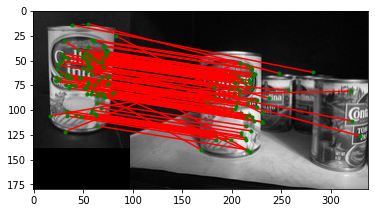
\includegraphics{results/q2_4.png}
\caption{img}
\end{figure}

BRIEF descriptors are not invariant to scale and rotational changes. So,
in case of same image being rotated or upscaled/downscaled, the
descriptors generated between these two images wouldn't match.

\begin{center}\rule{0.5\linewidth}{0.5pt}\end{center}

    \hypertarget{brief-and-rotations-5-pts}{%
\subsubsection{2.5 BRIEF and rotations (5
pts)}\label{brief-and-rotations-5-pts}}

Include your code and the historgram figure in your PDF, and explain why
you think the descriptor behaves this way.

    \begin{center}\rule{0.5\linewidth}{0.5pt}\end{center}

    \begin{tcolorbox}[breakable, size=fbox, boxrule=1pt, pad at break*=1mm,colback=cellbackground, colframe=cellborder]
\prompt{In}{incolor}{ }{\boxspacing}
\begin{Verbatim}[commandchars=\\\{\}]
\PY{n}{img1} \PY{o}{=} \PY{n}{cv2}\PY{o}{.}\PY{n}{imread}\PY{p}{(}\PY{l+s+s1}{\PYZsq{}}\PY{l+s+s1}{data/model\PYZus{}chickenbroth.jpg}\PY{l+s+s1}{\PYZsq{}}\PY{p}{)}
\PY{n}{locs1}\PY{p}{,} \PY{n}{desc1} \PY{o}{=} \PY{n}{briefLite}\PY{p}{(}\PY{n}{img1}\PY{p}{)}

\PY{n}{img2} \PY{o}{=} \PY{n}{cv2}\PY{o}{.}\PY{n}{imread}\PY{p}{(}\PY{l+s+s1}{\PYZsq{}}\PY{l+s+s1}{data/model\PYZus{}chickenbroth.jpg}\PY{l+s+s1}{\PYZsq{}}\PY{p}{)}   
\PY{n}{h}\PY{p}{,} \PY{n}{w}\PY{p}{,} \PY{n}{\PYZus{}} \PY{o}{=} \PY{n}{img2}\PY{o}{.}\PY{n}{shape}

\PY{n}{counts} \PY{o}{=} \PY{p}{[}\PY{p}{]}

\PY{k}{for} \PY{n}{i} \PY{o+ow}{in} \PY{n+nb}{range}\PY{p}{(}\PY{l+m+mi}{0}\PY{p}{,} \PY{l+m+mi}{370}\PY{p}{,} \PY{l+m+mi}{10}\PY{p}{)}\PY{p}{:}
    
    \PY{c+c1}{\PYZsh{} could\PYZsq{}ve just used this matrix again and again. However, the img2 quality is getting worse}
    \PY{c+c1}{\PYZsh{} so, matches are reducing.}
    \PY{n}{M} \PY{o}{=} \PY{n}{cv2}\PY{o}{.}\PY{n}{getRotationMatrix2D}\PY{p}{(}\PY{p}{(}\PY{n}{w} \PY{o}{/} \PY{l+m+mi}{2}\PY{p}{,} \PY{n}{h} \PY{o}{/} \PY{l+m+mi}{2}\PY{p}{)}\PY{p}{,} \PY{n}{i}\PY{p}{,} \PY{l+m+mf}{1.0}\PY{p}{)}
    \PY{n}{rotated} \PY{o}{=} \PY{n}{cv2}\PY{o}{.}\PY{n}{warpAffine}\PY{p}{(}\PY{n}{img2}\PY{p}{,} \PY{n}{M}\PY{p}{,} \PY{p}{(}\PY{n}{w}\PY{p}{,} \PY{n}{h}\PY{p}{)}\PY{p}{)}    
    \PY{n}{locs2}\PY{p}{,} \PY{n}{desc2} \PY{o}{=} \PY{n}{briefLite}\PY{p}{(}\PY{n}{rotated}\PY{p}{)}
    \PY{n}{matches} \PY{o}{=} \PY{n}{briefMatch}\PY{p}{(}\PY{n}{desc1}\PY{p}{,} \PY{n}{desc2}\PY{p}{)}
    
    \PY{n}{counts}\PY{o}{.}\PY{n}{append}\PY{p}{(}\PY{n+nb}{len}\PY{p}{(}\PY{n}{matches}\PY{p}{)}\PY{p}{)}
    
\PY{n}{plt}\PY{o}{.}\PY{n}{plot}\PY{p}{(}\PY{n+nb}{list}\PY{p}{(}\PY{n+nb}{range}\PY{p}{(}\PY{l+m+mi}{0}\PY{p}{,} \PY{l+m+mi}{370}\PY{p}{,} \PY{l+m+mi}{10}\PY{p}{)}\PY{p}{)}\PY{p}{,} \PY{n}{counts}\PY{p}{,} \PY{l+s+s1}{\PYZsq{}}\PY{l+s+s1}{ro\PYZhy{}}\PY{l+s+s1}{\PYZsq{}}\PY{p}{)}
\PY{n}{plt}\PY{o}{.}\PY{n}{xlabel}\PY{p}{(}\PY{l+s+s1}{\PYZsq{}}\PY{l+s+s1}{Angle of Rotation}\PY{l+s+s1}{\PYZsq{}}\PY{p}{)}
\PY{n}{plt}\PY{o}{.}\PY{n}{ylabel}\PY{p}{(}\PY{l+s+s1}{\PYZsq{}}\PY{l+s+s1}{\PYZsh{}Matches}\PY{l+s+s1}{\PYZsq{}}\PY{p}{)}
\PY{n}{plt}\PY{o}{.}\PY{n}{show}\PY{p}{(}\PY{p}{)}
\end{Verbatim}
\end{tcolorbox}

    \begin{figure}
\centering
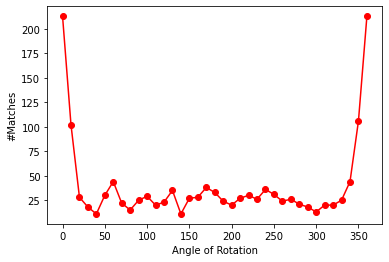
\includegraphics{results/q2_5.png}
\caption{img}
\end{figure}

The descriptor works by looking at n pairs of pixel in a patch around a
keypoint. However, because of rotation, the pixel locations have locally
changed within the patch. Thus, the n pairs are no longer referring to
the same pixels as the ones in the unrotated image.

\begin{center}\rule{0.5\linewidth}{0.5pt}\end{center}

    \hypertarget{improving-performance---extra-credit-10-pts}{%
\subsubsection{2.6 Improving Performance - (Extra Credit, 10
pts)}\label{improving-performance---extra-credit-10-pts}}

The extra credit opportunities described below are optional and provide
an avenue to explore computer vision and improve the performance of the
techniques developed above.

\begin{enumerate}
\def\labelenumi{\arabic{enumi}.}
\item
  (\(\textbf{5 pts}\)) As we have seen, BRIEF is not rotation invariant.
  Design a simple fix to solve this problem using the tools you have
  developed so far (think back to edge detection and/or Harris corner's
  covariance matrix). Include yout code in your PDF, and explain your
  design decisions and how you selected any parameters that you use.
  Demonstrate the effectiveness of your algorithm on image pairs related
  by large rotation.
\item
  (\(\textbf{5 pts}\)) This implementation of BRIEF has some scale
  invariance, but there are limits. What happens when you match a
  picture to the same picture at half the size? Look to section 3 of
  \href{https://www.cs.ubc.ca/~lowe/papers/ijcv04.pdf}{Lowe2004} for a
  technique that will make your detector more robust to changes in
  scale. Implement it and demonstrate it in action with several test
  images. Include yout code and the test images in your PDF. You may
  simply rescale some of the test images we have given you.
\end{enumerate}

    \begin{center}\rule{0.5\linewidth}{0.5pt}\end{center}

YOUR ANSWER HERE\ldots{}

\begin{center}\rule{0.5\linewidth}{0.5pt}\end{center}

    \hypertarget{automated-homography-estimationwarping-for-augmented-reality-10-points}{%
\subsubsection{3.3 Automated Homography Estimation/Warping for Augmented
Reality (10
points)}\label{automated-homography-estimationwarping-for-augmented-reality-10-points}}

Implement the following steps: 1. Reads $\texttt{cv_cover.jpg}$,
$\texttt{cv_desk.png}$, and $\texttt{hp_cover.jpg}$. 2. Computes a
homography automatically using $\texttt{computeH_ransac}$. 3. Warps
\(\texttt{hp_cover.jpg}\) to the dimensions of the
\(\texttt{cv_desk.png}\) image using the OpenCV
\(\texttt{warpPerspective}\) function. 4. At this point you should
notice that although the image is being warped to the correct location,
it is not filling up the same space as the book. Why do you think this
is happening? How would you modify \(\texttt{hp_cover.jpg}\) to fix this
issue? 5. Implement the function:
\(\texttt{function [ composite_img ] = compositeH( H2to1, template, img) }\)
to now compose this warped image with the desk image as in the following
figures. 6. Include your resulting image in your write-up. Please also
print the final H matrix in your writeup (normalized so the bottom right
value is 1)

    \begin{center}\rule{0.5\linewidth}{0.5pt}\end{center}

    \begin{tcolorbox}[breakable, size=fbox, boxrule=1pt, pad at break*=1mm,colback=cellbackground, colframe=cellborder]
\prompt{In}{incolor}{ }{\boxspacing}
\begin{Verbatim}[commandchars=\\\{\}]
\PY{k}{def} \PY{n+nf}{compositeH}\PY{p}{(}\PY{n}{H}\PY{p}{,} \PY{n}{template}\PY{p}{,} \PY{n}{img}\PY{p}{)}\PY{p}{:}
        
    \PY{n}{warped\PYZus{}img} \PY{o}{=} \PY{n}{cv2}\PY{o}{.}\PY{n}{warpPerspective}\PY{p}{(}\PY{n}{template}\PY{p}{,} \PY{n}{np}\PY{o}{.}\PY{n}{linalg}\PY{o}{.}\PY{n}{inv}\PY{p}{(}\PY{n}{H}\PY{p}{)}\PY{p}{,} \PY{n}{img}\PY{o}{.}\PY{n}{shape}\PY{p}{[}\PY{o}{\PYZhy{}}\PY{l+m+mi}{2}\PY{p}{:} \PY{o}{\PYZhy{}}\PY{l+m+mi}{4}\PY{p}{:} \PY{o}{\PYZhy{}}\PY{l+m+mi}{1}\PY{p}{]}\PY{p}{)}
    \PY{n}{composite\PYZus{}img} \PY{o}{=} \PY{n}{np}\PY{o}{.}\PY{n}{uint8}\PY{p}{(}\PY{n}{warped\PYZus{}img} \PY{o}{==} \PY{l+m+mi}{0}\PY{p}{)} \PY{o}{*} \PY{n}{img} \PY{o}{+} \PY{n}{warped\PYZus{}img}
    
    \PY{k}{return} \PY{n}{composite\PYZus{}img}\PY{o}{.}\PY{n}{astype}\PY{p}{(}\PY{n}{np}\PY{o}{.}\PY{n}{uint8}\PY{p}{)}

\PY{n}{im1} \PY{o}{=} \PY{n}{cv2}\PY{o}{.}\PY{n}{cvtColor}\PY{p}{(}\PY{n}{cv2}\PY{o}{.}\PY{n}{imread}\PY{p}{(}\PY{l+s+s2}{\PYZdq{}}\PY{l+s+s2}{figure/cv\PYZus{}cover.jpg}\PY{l+s+s2}{\PYZdq{}}\PY{p}{)}\PY{p}{,} \PY{n}{cv2}\PY{o}{.}\PY{n}{COLOR\PYZus{}BGR2RGB}\PY{p}{)}
\PY{n}{im2} \PY{o}{=} \PY{n}{cv2}\PY{o}{.}\PY{n}{cvtColor}\PY{p}{(}\PY{n}{cv2}\PY{o}{.}\PY{n}{imread}\PY{p}{(}\PY{l+s+s2}{\PYZdq{}}\PY{l+s+s2}{figure/cv\PYZus{}desk.png}\PY{l+s+s2}{\PYZdq{}}\PY{p}{)}\PY{p}{,} \PY{n}{cv2}\PY{o}{.}\PY{n}{COLOR\PYZus{}BGR2RGB}\PY{p}{)}

\PY{n}{locs1}\PY{p}{,} \PY{n}{desc1} \PY{o}{=} \PY{n}{briefLite}\PY{p}{(}\PY{n}{im1}\PY{p}{)}
\PY{n}{locs2}\PY{p}{,} \PY{n}{desc2} \PY{o}{=} \PY{n}{briefLite}\PY{p}{(}\PY{n}{im2}\PY{p}{)}
\PY{n}{matches} \PY{o}{=} \PY{n}{briefMatch}\PY{p}{(}\PY{n}{desc1}\PY{p}{,} \PY{n}{desc2}\PY{p}{)}

\PY{n}{H}\PY{p}{,} \PY{n}{inliers} \PY{o}{=} \PY{n}{computeH\PYZus{}ransac}\PY{p}{(}\PY{n}{matches}\PY{p}{,} \PY{n}{locs1}\PY{p}{,} \PY{n}{locs2}\PY{p}{)}

\PY{n+nb}{print}\PY{p}{(}\PY{l+s+s1}{\PYZsq{}}\PY{l+s+s1}{H: }\PY{l+s+si}{\PYZob{}0\PYZcb{}}\PY{l+s+s1}{\PYZsq{}}\PY{o}{.}\PY{n}{format}\PY{p}{(}\PY{n}{H} \PY{o}{/} \PY{n}{H}\PY{p}{[}\PY{l+m+mi}{2}\PY{p}{,} \PY{l+m+mi}{2}\PY{p}{]}\PY{p}{)}\PY{p}{)}

\PY{n}{template} \PY{o}{=} \PY{n}{cv2}\PY{o}{.}\PY{n}{cvtColor}\PY{p}{(}\PY{n}{cv2}\PY{o}{.}\PY{n}{imread}\PY{p}{(}\PY{l+s+s2}{\PYZdq{}}\PY{l+s+s2}{figure/hp\PYZus{}cover.jpg}\PY{l+s+s2}{\PYZdq{}}\PY{p}{)}\PY{p}{,} \PY{n}{cv2}\PY{o}{.}\PY{n}{COLOR\PYZus{}BGR2RGB}\PY{p}{)}

\PY{c+c1}{\PYZsh{} Resizing image to meet the im1 shape so that homography matrix works properly.}
\PY{n}{resized\PYZus{}template} \PY{o}{=} \PY{n}{cv2}\PY{o}{.}\PY{n}{resize}\PY{p}{(}\PY{n}{template}\PY{p}{,} \PY{n}{im1}\PY{o}{.}\PY{n}{shape}\PY{p}{[}\PY{o}{\PYZhy{}}\PY{l+m+mi}{2}\PY{p}{:} \PY{o}{\PYZhy{}}\PY{l+m+mi}{4}\PY{p}{:} \PY{o}{\PYZhy{}}\PY{l+m+mi}{1}\PY{p}{]}\PY{p}{)}

\PY{n}{composite\PYZus{}img} \PY{o}{=} \PY{n}{compositeH}\PY{p}{(}\PY{n}{H}\PY{p}{,} \PY{n}{resized\PYZus{}template}\PY{p}{,} \PY{n}{im2}\PY{p}{)}

\PY{n}{fig}\PY{p}{,} \PY{n}{axes} \PY{o}{=} \PY{n}{plt}\PY{o}{.}\PY{n}{subplots}\PY{p}{(}\PY{l+m+mi}{1}\PY{p}{,} \PY{l+m+mi}{3}\PY{p}{,} \PY{n}{figsize}\PY{o}{=}\PY{p}{(}\PY{l+m+mi}{15}\PY{p}{,} \PY{l+m+mi}{15}\PY{p}{)}\PY{p}{)}

\PY{n}{axes}\PY{p}{[}\PY{l+m+mi}{0}\PY{p}{]}\PY{o}{.}\PY{n}{imshow}\PY{p}{(}\PY{n}{im2}\PY{p}{)}
\PY{n}{axes}\PY{p}{[}\PY{l+m+mi}{0}\PY{p}{]}\PY{o}{.}\PY{n}{set\PYZus{}title}\PY{p}{(}\PY{l+s+s1}{\PYZsq{}}\PY{l+s+s1}{Text Book}\PY{l+s+s1}{\PYZsq{}}\PY{p}{)}
\PY{n}{axes}\PY{p}{[}\PY{l+m+mi}{1}\PY{p}{]}\PY{o}{.}\PY{n}{imshow}\PY{p}{(}\PY{n}{resized\PYZus{}template}\PY{p}{)}
\PY{n}{axes}\PY{p}{[}\PY{l+m+mi}{1}\PY{p}{]}\PY{o}{.}\PY{n}{set\PYZus{}title}\PY{p}{(}\PY{l+s+s1}{\PYZsq{}}\PY{l+s+s1}{Resized HP}\PY{l+s+s1}{\PYZsq{}}\PY{p}{)}
\PY{n}{axes}\PY{p}{[}\PY{l+m+mi}{2}\PY{p}{]}\PY{o}{.}\PY{n}{imshow}\PY{p}{(}\PY{n}{composite\PYZus{}img}\PY{p}{)}
\PY{n}{axes}\PY{p}{[}\PY{l+m+mi}{2}\PY{p}{]}\PY{o}{.}\PY{n}{set\PYZus{}title}\PY{p}{(}\PY{l+s+s1}{\PYZsq{}}\PY{l+s+s1}{Composite}\PY{l+s+s1}{\PYZsq{}}\PY{p}{)}
\PY{n}{plt}\PY{o}{.}\PY{n}{show}\PY{p}{(}\PY{p}{)}
\end{Verbatim}
\end{tcolorbox}

    \[H= \begin{bmatrix}
2.35252906e+00 & 6.88051228e-01 & -6.86719269e+02\\
1.01883048e-01 & 4.25832288e+00 & -8.42107269e+02\\
1.96661190e-04 & 3.70549187e-03 & 1.00000000e+00\\
 \end{bmatrix}\]

\begin{figure}
\centering
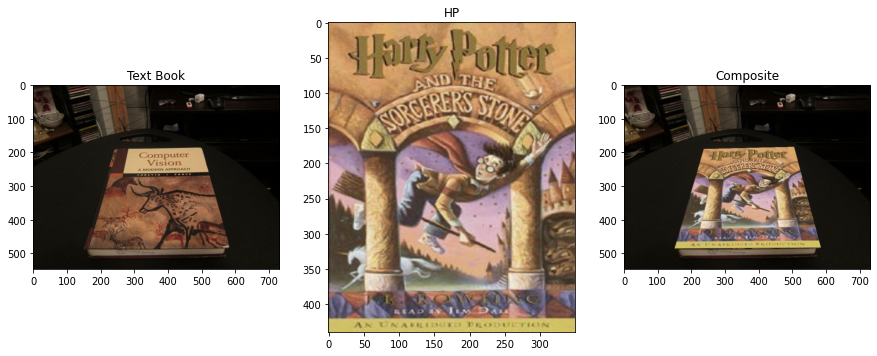
\includegraphics{results/q3_3.png}
\caption{img}
\end{figure}

\begin{center}\rule{0.5\linewidth}{0.5pt}\end{center}

    \hypertarget{image-stitching-5-pts}{%
\subsubsection{4.1 Image Stitching (5
pts)}\label{image-stitching-5-pts}}

Visualize the warped image. Please include the image and your H2to1
matrix (with the bottom right index as 1) in your writeup PDF, along
with stating which image pair you used.

    \begin{center}\rule{0.5\linewidth}{0.5pt}\end{center}

    \begin{tcolorbox}[breakable, size=fbox, boxrule=1pt, pad at break*=1mm,colback=cellbackground, colframe=cellborder]
\prompt{In}{incolor}{ }{\boxspacing}
\begin{Verbatim}[commandchars=\\\{\}]
\PY{k}{def} \PY{n+nf}{imageStitching}\PY{p}{(}\PY{n}{im1}\PY{p}{,} \PY{n}{im2}\PY{p}{,} \PY{n}{H2to1}\PY{p}{,} \PY{n}{pad}\PY{o}{=}\PY{p}{(}\PY{p}{(}\PY{l+m+mi}{0}\PY{p}{,} \PY{l+m+mi}{0}\PY{p}{)}\PY{p}{,} \PY{p}{(}\PY{l+m+mi}{0}\PY{p}{,} \PY{l+m+mi}{500}\PY{p}{)}\PY{p}{,} \PY{p}{(}\PY{l+m+mi}{0}\PY{p}{,} \PY{l+m+mi}{0}\PY{p}{)}\PY{p}{)}\PY{p}{)}\PY{p}{:}
    \PY{l+s+sd}{\PYZsq{}\PYZsq{}\PYZsq{}}
\PY{l+s+sd}{    Returns a panorama of im1 and im2 using the given }
\PY{l+s+sd}{    homography matrix}

\PY{l+s+sd}{    INPUT}
\PY{l+s+sd}{        Warps img2 into img1 reference frame using the provided warpH() function}
\PY{l+s+sd}{        H2to1 \PYZhy{} a 3 x 3 matrix encoding the homography that best matches the linear}
\PY{l+s+sd}{                 equation.}
\PY{l+s+sd}{    OUTPUT}
\PY{l+s+sd}{        img\PYZus{}pano \PYZhy{} the panorama image.}
\PY{l+s+sd}{    \PYZsq{}\PYZsq{}\PYZsq{}}
    
    \PY{n}{padded\PYZus{}im1} \PY{o}{=} \PY{n}{np}\PY{o}{.}\PY{n}{pad}\PY{p}{(}\PY{n}{im1}\PY{p}{,} \PY{n}{pad}\PY{p}{)}    
    \PY{n}{warped\PYZus{}img} \PY{o}{=} \PY{n}{cv2}\PY{o}{.}\PY{n}{warpPerspective}\PY{p}{(}\PY{n}{im2}\PY{p}{,} \PY{n}{H2to1}\PY{p}{,} \PY{n}{padded\PYZus{}im1}\PY{o}{.}\PY{n}{shape}\PY{p}{[}\PY{o}{\PYZhy{}}\PY{l+m+mi}{2}\PY{p}{:} \PY{o}{\PYZhy{}}\PY{l+m+mi}{4}\PY{p}{:} \PY{o}{\PYZhy{}}\PY{l+m+mi}{1}\PY{p}{]}\PY{p}{)}
    
    \PY{c+c1}{\PYZsh{} Generating weights for alpha blending.}
    \PY{n}{w1} \PY{o}{=} \PY{n}{distance\PYZus{}transform\PYZus{}edt}\PY{p}{(}\PY{n}{np}\PY{o}{.}\PY{n}{pad}\PY{p}{(}\PY{n}{np}\PY{o}{.}\PY{n}{ones\PYZus{}like}\PY{p}{(}\PY{n}{im1}\PY{p}{[}\PY{l+m+mi}{1}\PY{p}{:} \PY{o}{\PYZhy{}}\PY{l+m+mi}{1}\PY{p}{,} \PY{l+m+mi}{1}\PY{p}{:} \PY{o}{\PYZhy{}}\PY{l+m+mi}{1}\PY{p}{,} \PY{l+m+mi}{0}\PY{p}{]}\PY{p}{)}\PY{p}{,} \PY{l+m+mi}{1}\PY{p}{)}\PY{p}{)}
    \PY{n}{w2} \PY{o}{=} \PY{n}{distance\PYZus{}transform\PYZus{}edt}\PY{p}{(}\PY{n}{np}\PY{o}{.}\PY{n}{pad}\PY{p}{(}\PY{n}{np}\PY{o}{.}\PY{n}{ones\PYZus{}like}\PY{p}{(}\PY{n}{im2}\PY{p}{[}\PY{l+m+mi}{1}\PY{p}{:} \PY{o}{\PYZhy{}}\PY{l+m+mi}{1}\PY{p}{,} \PY{l+m+mi}{1}\PY{p}{:} \PY{o}{\PYZhy{}}\PY{l+m+mi}{1}\PY{p}{,} \PY{l+m+mi}{0}\PY{p}{]}\PY{p}{)}\PY{p}{,} \PY{l+m+mi}{1}\PY{p}{)}\PY{p}{)}
    
    \PY{c+c1}{\PYZsh{} Padding w1 as required to maintain right weight distribution.}
    \PY{n}{padded\PYZus{}w1} \PY{o}{=} \PY{n}{np}\PY{o}{.}\PY{n}{pad}\PY{p}{(}\PY{n}{w1}\PY{p}{,} \PY{n}{pad}\PY{p}{[}\PY{l+m+mi}{0}\PY{p}{:} \PY{l+m+mi}{2}\PY{p}{]}\PY{p}{)} 
    \PY{n}{padded\PYZus{}w1} \PY{o}{=} \PY{n}{padded\PYZus{}w1}\PY{o}{.}\PY{n}{reshape}\PY{p}{(}\PY{n}{padded\PYZus{}w1}\PY{o}{.}\PY{n}{shape}\PY{p}{[}\PY{l+m+mi}{0}\PY{p}{]}\PY{p}{,} \PY{o}{\PYZhy{}}\PY{l+m+mi}{1}\PY{p}{,} \PY{l+m+mi}{1}\PY{p}{)}
    
    \PY{c+c1}{\PYZsh{} Warping weights for im2 to the target shape.}
    \PY{n}{warped\PYZus{}w2} \PY{o}{=} \PY{n}{cv2}\PY{o}{.}\PY{n}{warpPerspective}\PY{p}{(}\PY{n}{w2}\PY{p}{,} \PY{n}{H2to1}\PY{p}{,} \PY{n}{padded\PYZus{}im1}\PY{o}{.}\PY{n}{shape}\PY{p}{[}\PY{o}{\PYZhy{}}\PY{l+m+mi}{2}\PY{p}{:} \PY{o}{\PYZhy{}}\PY{l+m+mi}{4}\PY{p}{:} \PY{o}{\PYZhy{}}\PY{l+m+mi}{1}\PY{p}{]}\PY{p}{)}
    \PY{n}{warped\PYZus{}w2} \PY{o}{=} \PY{n}{warped\PYZus{}w2}\PY{o}{.}\PY{n}{reshape}\PY{p}{(}\PY{n}{warped\PYZus{}w2}\PY{o}{.}\PY{n}{shape}\PY{p}{[}\PY{l+m+mi}{0}\PY{p}{]}\PY{p}{,} \PY{o}{\PYZhy{}}\PY{l+m+mi}{1}\PY{p}{,} \PY{l+m+mi}{1}\PY{p}{)}
    
    \PY{n}{img\PYZus{}pano} \PY{o}{=} \PY{n}{np}\PY{o}{.}\PY{n}{uint8}\PY{p}{(}\PY{p}{(}\PY{n}{padded\PYZus{}im1} \PY{o}{*} \PY{n}{padded\PYZus{}w1} \PY{o}{+} \PY{n}{warped\PYZus{}img} \PY{o}{*} \PY{n}{warped\PYZus{}w2}\PY{p}{)} \PY{o}{/} \PY{p}{(}\PY{n}{padded\PYZus{}w1} \PY{o}{+} \PY{n}{warped\PYZus{}w2}\PY{p}{)}\PY{p}{)}
    
    \PY{k}{return} \PY{n}{img\PYZus{}pano}
\end{Verbatim}
\end{tcolorbox}

    \[H2to1= \begin{bmatrix}
6.50985010e-01 & -4.40168516e-02 & 3.65903823e+02\\
-7.99527543e-02 & 8.72003506e-01 & -1.59370556e+01\\
-3.55709534e-04 & -1.73167455e-05 & 1.00000000e+00\\
 \end{bmatrix}\]

Image1 \includegraphics{data/incline_L.png}

Image2 \includegraphics{data/incline_R.png}

Stitched Image 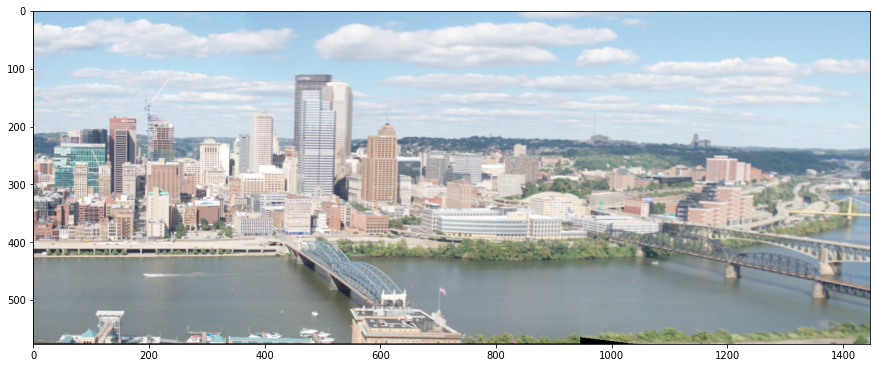
\includegraphics{results/q4_1.png}

\begin{center}\rule{0.5\linewidth}{0.5pt}\end{center}

    \hypertarget{image-stitching-with-no-clip-3-pts}{%
\subsubsection{4.2 Image Stitching with No Clip (3
pts)}\label{image-stitching-with-no-clip-3-pts}}

Visualize the warped image. Please include the image in your writeup
PDF, along with stating which image pair you used.

    \begin{center}\rule{0.5\linewidth}{0.5pt}\end{center}

Image1 \includegraphics{data/incline_L.png}

Image2 \includegraphics{data/incline_R.png}

Stitched Image 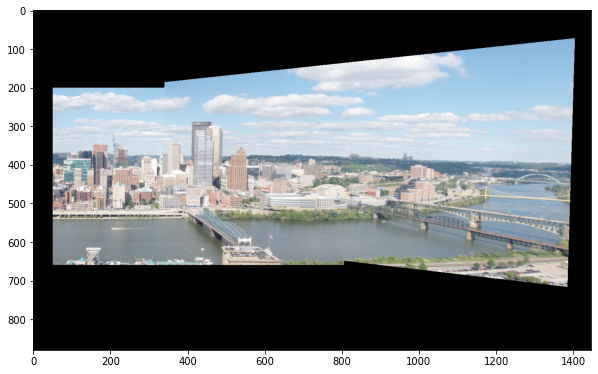
\includegraphics{results/q4_2.png}

\begin{center}\rule{0.5\linewidth}{0.5pt}\end{center}

    \hypertarget{generate-panorama-2-pts}{%
\subsubsection{4.3 Generate Panorama (2
pts)}\label{generate-panorama-2-pts}}

Save the resulting panorama on the full sized images and include the
figure and computed homography matrix in your writeup.

    \begin{center}\rule{0.5\linewidth}{0.5pt}\end{center}

\[H2to1= \begin{bmatrix}
6.70688040e-01 & -3.24766846e-02 & 3.61588728e+02\\
-7.62290199e-02 & 8.90118506e-01 & -2.09211372e+01\\
-3.42501786e-04 & -2.92305590e-06 & 1.00000000e+00\\
 \end{bmatrix}\]

Panorama 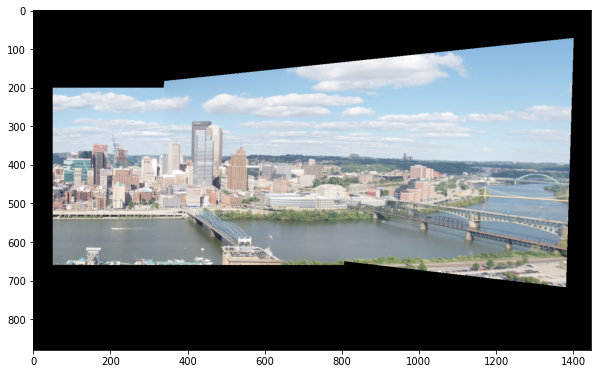
\includegraphics{results/q4_3.png}

\begin{center}\rule{0.5\linewidth}{0.5pt}\end{center}

    \hypertarget{extra-credits-3-pts}{%
\subsubsection{4.4 extra credits (3 pts)}\label{extra-credits-3-pts}}

Collect a pair of your own images (with your phone) and stitch them
together using your code from the previous section. Include the pair of
images and their result in the write-up.

    \begin{center}\rule{0.5\linewidth}{0.5pt}\end{center}

\begin{figure}
\centering
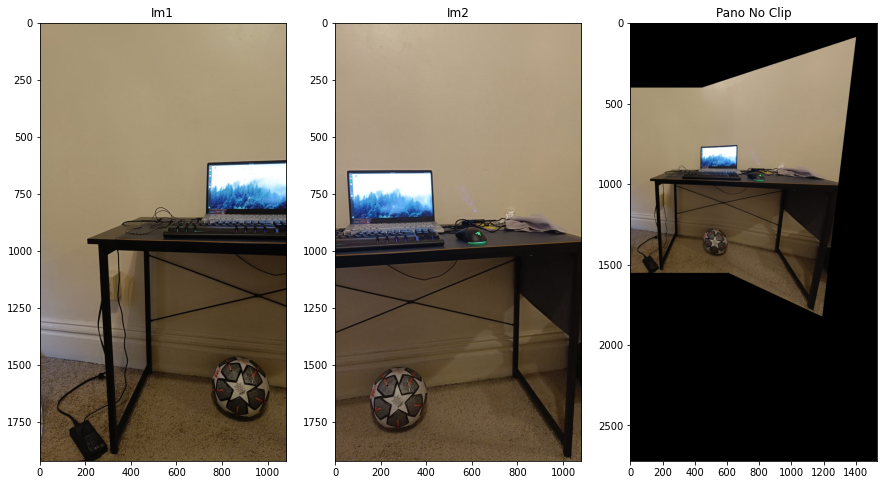
\includegraphics{results/q4_4.png}
\caption{img}
\end{figure}

\begin{center}\rule{0.5\linewidth}{0.5pt}\end{center}

    \hypertarget{extra-credits-2-pts}{%
\subsubsection{4.5 extra credits (2 pts)}\label{extra-credits-2-pts}}

Collect at least 6 images and stitch them into a single noClip image.
You can either collect your own, or use the
\href{http://www.cs.jhu.edu/~misha/Code/SMG/PNC3.zip}{PNC Park images}
from Matt Uyttendaele. We used the PNC park images (subsmapled to 1/4
sized) and ORB keypoints and descriptors for our reference solution.

    \begin{center}\rule{0.5\linewidth}{0.5pt}\end{center}

YOUR ANSWER HERE\ldots{}

\begin{center}\rule{0.5\linewidth}{0.5pt}\end{center}

    \hypertarget{question-5-poisson-image-stitching-15-points}{%
\subsection{Question 5: Poisson Image Stitching (15
points)}\label{question-5-poisson-image-stitching-15-points}}

Write a function called
\(\texttt{poisson_blend(background,foreground,mask)}\) which takes 3
equal sized images (background and foreground as RGB, mask as binary)
and solves the Poisson equation, using gradients from foreground and
boundary conditions from the background.

\textbf{The problem will be manually graded.} Please include results
from both the \(\texttt{(fg1,bg1,mask1)}\) and
\(\texttt{(fg2,bg2,mask2)}\) images in your write-up.

    \begin{center}\rule{0.5\linewidth}{0.5pt}\end{center}

YOUR ANSWER HERE\ldots{}

\begin{center}\rule{0.5\linewidth}{0.5pt}\end{center}


    % Add a bibliography block to the postdoc
    
    
    
\end{document}
